
\chapter{Time Seriers Rumor Detection Model} % (fold)
\label{cha:timr_seriers_rumor_model}
As we showed in figures \ref{fig:Url5000} and \ref{fig:largecity}, The fraction of tweets containing url with top 5000 domain and the fraction of poster living in large city which are both constantly changing. In order to capture these changes of the each features we use Dynamic Series-Time Structure (DSTS) which was presented in Ma's work \cite{ma2015detect}. In the an Event $E_{i}$ there is a set of tweets $tw_{ij}$ and we split them into different time intervals according to the creation time so that we can analyze the features in time series. We test the different classifiers with this model, we compare it with static features and in the end we rank all features and show their performance over time.

\begin{figure}[!h]
\centering
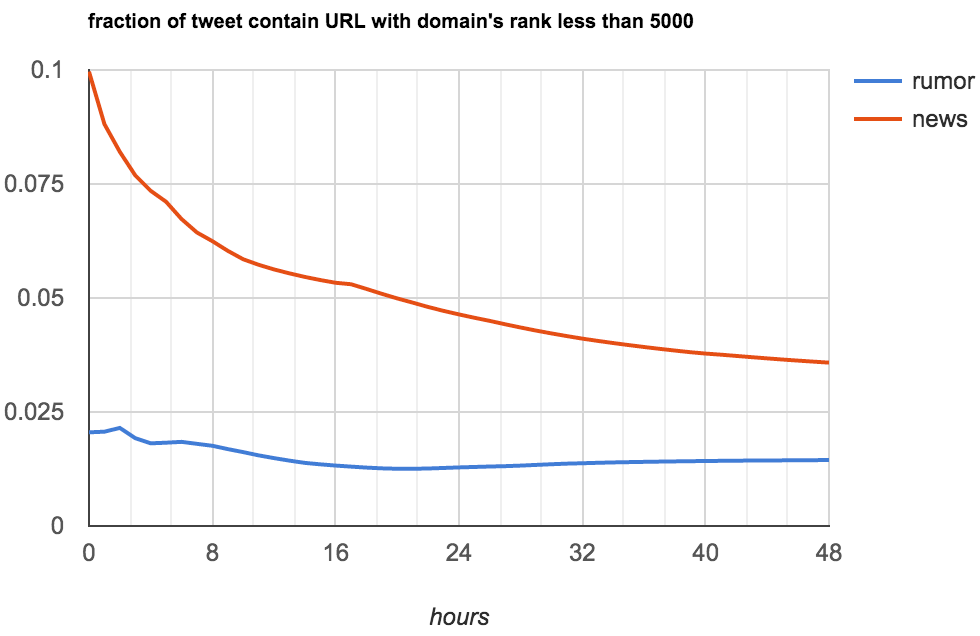
\includegraphics[width=0.52\columnwidth]{images/url5000.png}
\caption{The fraction of tweets containing url with top 5000 domain}
\label{fig:Url5000}
\end{figure}
\begin{figure}[!h]
\centering
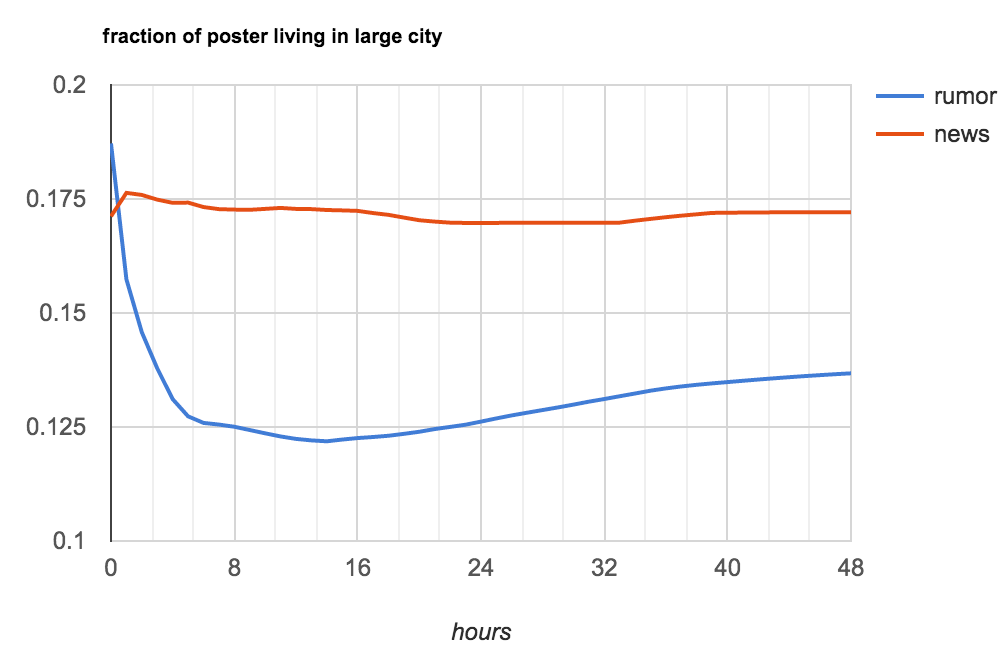
\includegraphics[width=0.52\columnwidth]{images/largecity.png}
\caption{The fraction of poster living in large city}
\label{fig:largecity}
\end{figure}
\newpage
  \section{ Dynamic Series-Time Structure (DSTS)} 
   \subsection{Time Stamps Generation} 
   For an event $E_i$ we define $timeFirst_i$ as the start time of the event, $timeFirst_i$ as the time of last tweet of the event. We split the each tweet $tw_{ij}$ into N time intervals according to the creation time. The length of each time interval we define as follow: 
   
\begin{equation}
Interval(E_i)=\frac{\left \lceil { (timeLast_i-timeFirst_i) }\right \rceil}{N}
\end{equation}
And the index of time interval $TS(t_{ij})$ where a tweet $tw_{ij}$ which is created in time $t_{ij}$ should fall into, we define as follow :

\begin{equation}
TS(t_{ij})=\frac{\left \lfloor { (t_{ij}-timeFirst_i) }\right \rfloor}{Interval(E_i)}
\end{equation}

In our work $Interval(E_i)$ as we defined in section \ref{sec:Time_Period_of_an_Event} is one hour and N is constant 48 hours for each event.  
   
   \subsection{ Dynamic Series-Time Structure (DSTS)} 
Now we have all the time intervals of an event $E_i$ and we can generate a vector V($E_i$ ) of features in each time interval. And in order to capture the changes of feature over time we should no only model the features in individual time intervals but also we should model their difference between two time intervals. So the model of  DSTS is represented as:  

\begin{equation}
 V(E_i)=(\textbf{F}^D_{i,0}, \textbf{F}^D_{i,1},..., \textbf{F}^D_{i,N},\textbf{S}^D_{i,1},..., \textbf{S}^D_{i,N})
\end{equation}
where the $\textbf{F}^D_{i,t}$ is the feature vector in time interval t of event $E_i$.  $\textbf{S}^D_{i,t}$ is the difference between $\textbf{F}^D_{i,t}$ and $\textbf{F}^D_{i,t+1}$. V($E_i$ ) is the time series feature vector of the event $E_i$.
\begin{equation}
\textbf{F}^D_{i,t}=(\widetilde{ f}_{i,t,1},\widetilde{ f}_{i,t,2},...,\widetilde{ f}_{i,t,D})
\end{equation}

\begin{equation}
\textbf{S}^D_{i,t}=\frac{\textbf{F}^D_{i,t+1}-\textbf{F}^D_{i,t}}{Interval(E_i)}
\end{equation}
We use Z-score to normalize feature values which is implemented by sklearn.
\begin{equation}
\widetilde{f}_{i,t,k}=\frac{f_{i,t+1,k}-\overline{f}_{i,k}}{\sigma(f_{i,k})}
\end{equation}
where $f_{i,t,k}$ is the k-th feature in time interval t of the event $E_i$ in time interval t. $\overline{f}_{i,k}$ is the mean of the feature k of the event $E_i$ and $sigma(f_{i,k})$ is the standard deviation of the feature k over all time intervals. We skip this step when we use random forest and Decision Trees because they do not need feature normalization.

  \section{ Features} 
 
 We use a collection of features based on previous works  
\cite{castillo2011information}\cite{gupta2014tweetcred} \cite{yang2012automatic}\cite{liu2015real}\cite{madetecting}\cite{mendoza2010twitter}\cite{ma2015detect}\cite{wu2015false}\cite{jin2013epidemiological}. They are totally 50 features shown in table \ref{tab:full_features}. These features are not only extracted from Twitter interface but also other external websites like bluecoat.com which are mentioned in section \ref{cha:Data_Collection}. 
\subsection{Text Features}
Text features is normal feature set of tweets' content. It contains 16 features as shown in table \ref{tab:full_features}. The difference of the text features in single tweet model and in time series model is in time series model we use the percent of tweets which contain some attributes or average number of some attributes. 

NumOfChar is the average number of individual characters of tweets, it is case sensitivity. The average number of characters of rumor is 34 and news is 36.
\subsection{Twitter Features}
Twitter features is the features of Twitter's functions like Hashtag and mention.
And we add 3 features of the URLs of the tweets. The first one is the WOT Score which is crawled from the website wot.com \footnote{https://www.mywot.com/en/api}. WOT is short for Web of Trust and it scores the domains' credibility and safety. It offers API for developer. The second one is catalog of domain which I crawled from the bluecoat.com \footnote{http://sitereview.bluecoat.com/}. I group them into 2 parts news website or not. The last one is the rank of the domain which I crawled from alexa.com\footnote{http://www.alexa.com/siteinfo/bbc.com}. I also split them into 2 group rank less than 5000 or not. In our experiment those 3 feature about URL is better than others original Twitter functions like hashtag or mention.
\subsection{User Features}
User's features is similar with others works. We add one feature which can only get from the website interface is how many photos has the user posted (UserNumPhoto). It is in the BestSet of features. And one other user feature is if the user lives in a large city. We got the list of large city in the report of demographia\footnote{http://www.demographia.com/db-worldua.pdf}. It is also a good feature contained in the Bestset.
\subsection{Epidemiological Modeling Features}
\label{sec:epide}
Jin's work is as far as we know the first people using epidemiological model to analyze rumors' prorogation on twitter \cite{jin2013epidemiological}. They fits the volume of the rumors and news events into two models SIS (Susceptible, Infected, Susceptible) and SEIZ (susceptible, exposed, infected, skeptic). 

\textbf{SIS} is one of the most popular epidemiological model. To adapt to the scenario of Twitter, we define a user who posts a tweet of relevant event as \textbf{(I)} infected, a user who didn't we define as \textbf{(S)} susceptible. But unlikely as a normal epidemiological scenario infected nodes can be cured and return to be susceptible,  the user once posts a tweet of the certain events, he will be classified into the infected component forever. He can't be return susceptible class. At time t the total number of population is $\Delta N(t)= I(t) + S(t)$ where $I(t)$ is the size of infected population and  $S(t)$ is the size of susceptible population.  As shown in Figure \ref{fig:SIS}, SIS model works as follow:

\begin{figure}[!h]
\center
\def\layersep{2.5cm}
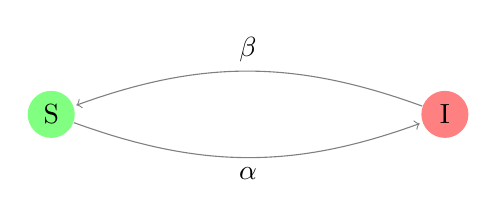
\begin{tikzpicture}[shorten >=1pt,->,draw=black!50, node distance=\layersep]
    \tikzstyle{every pin edge}=[<-,shorten <=1pt]
    \tikzstyle{neuron}=[circle,fill=black!25,minimum size=17pt,inner sep=0pt]
    \tikzstyle{input neuron}=[neuron, fill=green!50];
    \tikzstyle{output neuron}=[neuron, fill=red!50];
    % Draw the input layer nodes
     % This is the same as writing \foreach \name / \y in {1/1,2/2,3/3,4/4}
      \node[input neuron] (S) at (0,-1) {S};
     \node[ output neuron,  xshift=5cm,yshift=-1cm] (I) {I};
      \path  (I) edge [above, bend right=20]node [sloped,midway,above] {$\beta$} (S) ;
     \path  (S) edge [below, bend right=20] node [sloped,midway,below]{$\alpha $}(I) ;
    % Annotate the layers
 \end{tikzpicture}
   \caption{SIS Model}
\label{fig:SIS}
\end{figure}
	
\begin{itemize}
\item A user who posts tweets about the certain event is regarded as infected.
\item A susceptible user has not tweeted about the certain event
\item A susceptible user may see the a tweet about the certain event from a infected users and he immediately retweets or posts a tweet about this events, and in that he turns himself to infected.
\item Susceptible user will remain susceptible until he contacts (via tweet) with infected person.
\end{itemize}
we show SIS model mathematical as follow:
\begin{equation}
\frac{d[S]}{dt}=- \beta SI+\alpha I
\end{equation}
\begin{equation}
\frac{d[I]}{dt}= \beta SI-\alpha I
\end{equation}

SIS model assumes that a susceptible user once exposed to a infected user turns to infected immediately. That is one reason of this model why it didn't fit to Twitter. If fact when twitter users see a tweet they have their normal senesce to judgment the truth of the information and they can decide wether  further spreading the tweet or ignoring them.

Another popular model is SIR which contains one more term than the SIS. The definitions of \textbf{(S)} and \textbf{(I)} are the same of SIS but the term \textbf{(R)} stands for recover. Once a susceptible user is recover, he will be removed from the susceptible component and he can't be infected again. But we can't get a reasonable explanation of the term R if we model the an event spreading on Twitter.

Because of the Shortcomings of above two model, they test another model called SEIZ which reference from \cite{bettencourt2006power} . 
\begin{figure}[!h]
\center
\def\layersep{2.5cm}
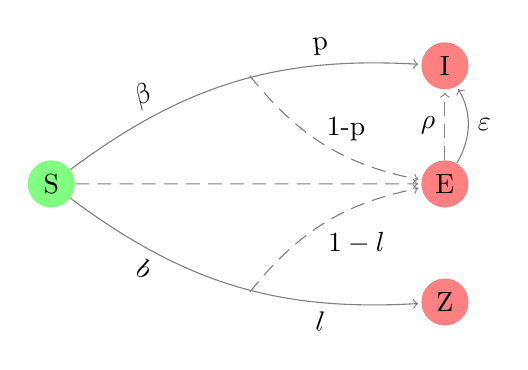
\begin{tikzpicture}[shorten >=1pt,->,draw=black!50, node distance=\layersep]
    \tikzstyle{every pin edge}=[<-,shorten <=1pt]
    \tikzstyle{neuron}=[circle,fill=black!25,minimum size=17pt,inner sep=0pt]
    \tikzstyle{input neuron}=[neuron, fill=green!50];
    \tikzstyle{output neuron}=[neuron, fill=red!50];
    \tikzstyle{miss node}=[inner sep=0,minimum size=1];
    % Draw the input layer nodes
     % This is the same as writing \foreach \name / \y in {1/1,2/2,3/3,4/4}
      \node[input neuron] (S) at (0,-2.5) {S};
      \node[ output neuron,  xshift=5cm,yshift=-1cm] (I) {I};
      \node[ output neuron,  xshift=5cm,yshift=-2.5cm] (E) {E};
      \node[ output neuron,  xshift=5cm,yshift=-4cm] (Z) {Z};
       \node[ miss node,  xshift=2.5cm,yshift=-1.1cm] (X) {};
       \node[ miss node,  xshift=2.5cm,yshift=-3.9cm] (X2) {};

	\path  (X) edge [dash pattern=on5pt off3pt,below, bend right=20] node [midway,right,xshift=-0.1cm,yshift=0.2cm]{1-p}(E) ;
 
      \path  (S) edge [above, bend left=20]node [sloped,near start,above] {$\beta$} node [sloped,near end,above] {p}  (I) ;
      \path  (E) edge [right, bend right=30] node [midway,right]{$\varepsilon $}(I) ;
      \path  (E) edge [dash pattern=on5pt off3pt] node [midway,left]{$\rho$}(I) ;
      \path  (S) edge [dash pattern=on5pt off3pt]  (E) ;
      \path  (S) edge [above, bend right=20]node [sloped,near start,below] {$b$} node [sloped,near end,below] {$l$}  (Z) ;
	\path  (X2) edge [dash pattern=on5pt off3pt,below, bend left=20] node [xshift=0.4cm]{$1-l $}(E) ;
	\end{tikzpicture}
   \caption{SEIZ Model}
\label{fig:SEIZ}
\end{figure}
 To adapt to Twitter context, the compartments of the SEIZ model can be mapped like this: \textbf{(S)} Susceptible is a user who has not been exposed to the event aka he didn't see any tweets about the certain event yet, \textbf{(I)} infected  means a user has posted tweets about the certain events, \textbf{(Z)} skeptic is a user who has been exposed to the certain event but he decides to ignore it and \textbf{(E)} exposed is a user who been exposed to the certain event but he will post the tweets after some delay.
 
 We show the model in figure \ref{fig:SEIZ}. And the SEIZ works as follow:
 

 \begin{itemize}
\item People recruit from \textbf{(S)} Susceptible compartment to Skeptics with rate b. But with probability l some of them directly deny the events and turn to \textbf{(Z)} skeptic compartments. Others  with probability 1-l probability turn to \textbf{(E)} exposed compartment.
\item People recruit from \textbf{(S)} Susceptible compartment to Infected with rate $\beta$. But with probability p some of them directly believe the events and repost it and turn them to be \textbf{(Z)} skeptic compartments. Others  with probability 1-p probability turn to \textbf{(E)} exposed compartment.
\item  People from \textbf{(E)} exposed compartment have $\rho$ probability contacting again with the Infected and turn them to \textbf{(I)} infected compartment. And others have $\varepsilon$ probability turn into \textbf{(I)} infected compartment by themselves for example external shock.
\end{itemize}



And we show the model mathematical like:
we show SEIZ model mathematical as follow:
\begin{equation}
\frac{d[S]}{dt}=- \beta S\frac{I}{N}- b S\frac{Z}{N}
\end{equation}
\begin{equation}
\frac{d[E]}{dt}=(1-p)\beta S\frac{I}{N}+(1-l) b S\frac{I}{N}-\rho  S\frac{Z}{N}-\varepsilon E
\end{equation}
\begin{equation}
\frac{d[I]}{dt}=p\beta S\frac{I}{N}+\rho  S\frac{Z}{N}+\varepsilon E
\end{equation}
\begin{equation}
\frac{d[Z]}{dt}=lbS\frac{Z}{N} 
\end{equation}

\begin{table*}[!h]
 \centering
\scalebox{1}{
\begin{tabular}{@{\textbf{ }}lllllll@{}}
\toprule
\textbf{Symbol} & \textbf{Definition} \\ \midrule
$\beta$ & S-I contact rate\\  
b	&	 S-Z contact rate\\
$\rho $	&	E-I contact rate\\ 
$\varepsilon $   &	Incubation rate\\
$1/ \varepsilon $   &	Average Incubation Time\\
bl	&	Effective rate of S -> Z\\ 
$\beta \rho$   &	Effective rate of S -> I\\
b(1-l) & Effective rate of S -> E via contact with Z\\
$\beta (1-p)$	&	 Effective rate of S -> E via contact with I\\ 
l   &	 S->Z Probability given contact with skeptics\\
1-l &  S->E Probability given contact with skeptics\\
p	&	S->I Probability given contact with adopters\\
1-p	&	S->E Probability given contact with adopters \\ \bottomrule
\end{tabular}}
\caption{Parameters of SEIZ}
\label{tab:SEIZ_Para}
\end{table*}
The author presents an index of SEIZ called $R_{SI}$ as equation \ref{RSI}. It contains all rate values of SEIZ and related to the flux ratio of the \textbf{(E)} exposed compartment, the ratio of entering \textbf{(E)} to leaving \textbf{(E)}. If $R_{SI}$ is bigger than 1 means the influx of exposed compartment is bigger than the efflux. This index may be a good candidate of feature to analyze rumor spreading on Twitter.


\begin{equation}
\label{RSI}
R_{SI}=\frac{(1-p)\beta+(1-l)b}{\rho+\varepsilon}  
\end{equation}

We use Levenberg-Marquard algorithm which we present in section \ref{sec:LM} to learn the parameters of the SIS and SPEI. The fitting data is the tweet volume of the 260 events  (130 rumors and 130 news). 
 In time each interval from $t_0$ to $t_n$, we fit the sequenced  tweet volume from the beginning time the $t_0$ to the current time interval $t_n$ of an event to SIS and SEIZ model and learn. From SIS we get two feature $\beta_{n},\alpha_{n}$ and from SEIZ we get 7 features $\beta_{n},b_{n},l_{n},p_{n},\varepsilon_{n},\rho_{n},RSI_{n}$. We add them into our DSTS.
 
$FittingFunction_{SIS}(TweetVolume_{0},...,TweetVolume_{n})$->$\beta_{n},\alpha_{n}$%


$FittingFunction_{SEIZ}(TweetVolume_{0},...,TweetVolume_{n})$->$\beta_{n},b_{n},l_{n},p_{n},\varepsilon_{n},\rho_{n},RSI_{n}$

 We show 4 examples as following two rumors in figure \ref{fig:SIS-rumor1} \ref{fig:SIS-rumor2} and two news in figure \ref{fig:SIS-news1}  \ref{fig:SIS-news2}. It is obvious that SEIZ is more appropriate than SIS to model in our Twitter application, because the fitting error of SPEI is less than SIS. 


\begin{figure}[!h]

  \centering

\subfigure[SIS and SEIZ model for rumor 1]{\label{fig:SIS-rumor1}
\centering
  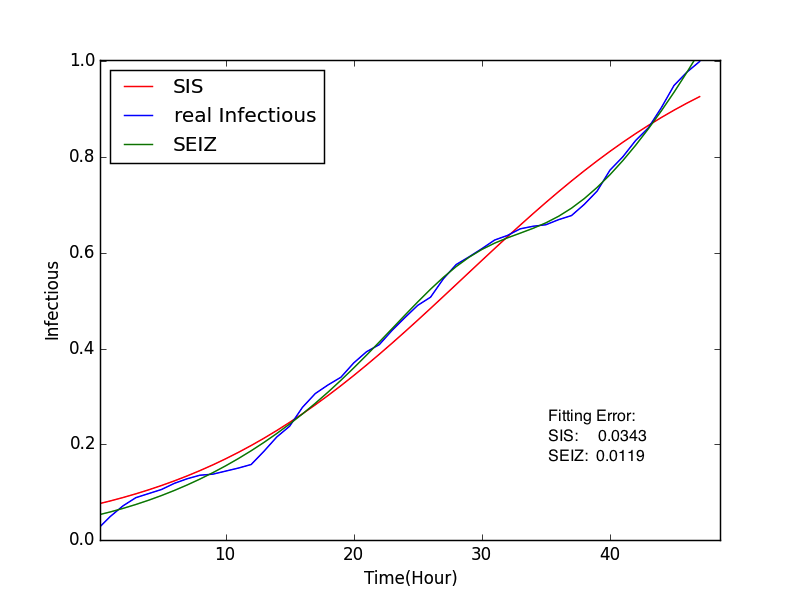
\includegraphics[width=0.48\columnwidth]{images/SISKKK.png}
} %
\subfigure[SIS and SEIZ model for rumor 2]{\label{fig:SIS-rumor2}
\centering
  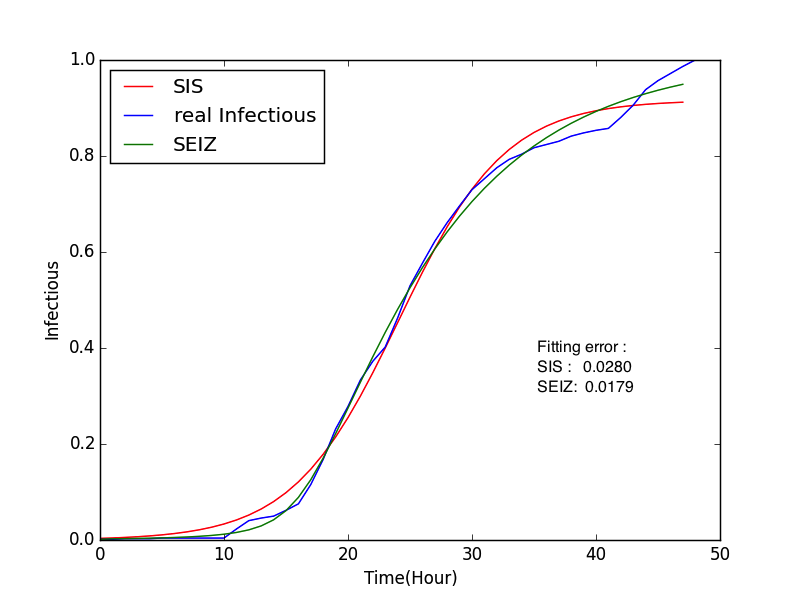
\includegraphics[width=0.48\columnwidth]{images/SIS449.png}
}
\subfigure[SIS and SEIZ model for news 1]{\label{fig:SIS-news1}
\centering
  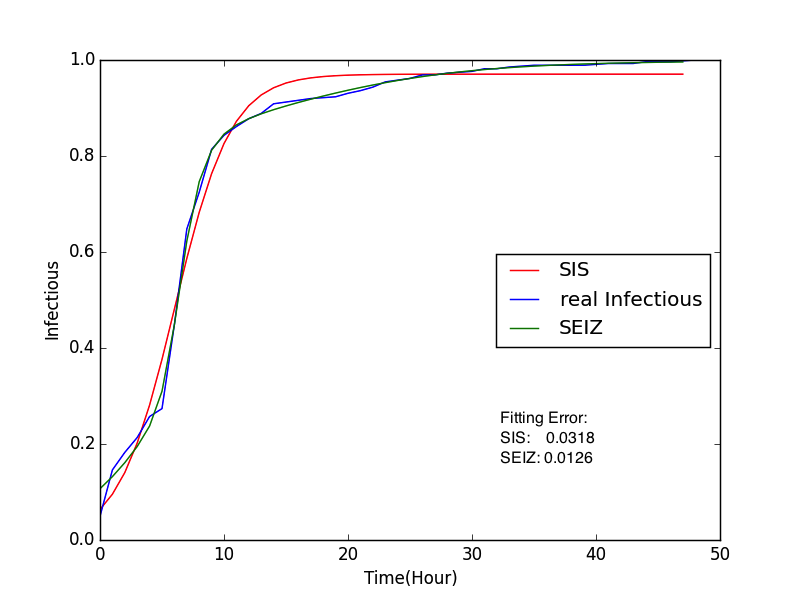
\includegraphics[width=0.48\columnwidth]{images/SISSHUMA.png}
}
\subfigure[SIS and SEIZ model for news 2]{\label{fig:SIS-news2}
\centering
  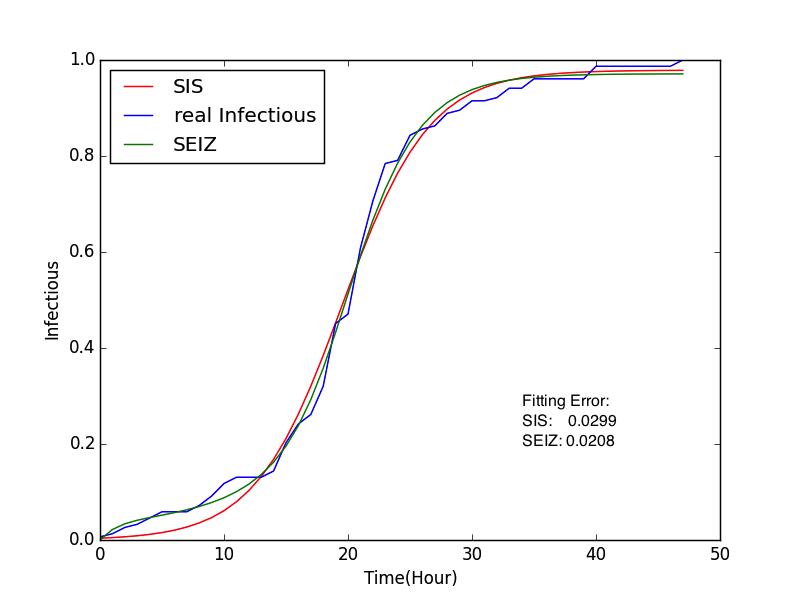
\includegraphics[width=0.48\columnwidth]{images/SIS1347.png}
}
\caption{Fitting results of SIS and SEIZ model of (a) Rumor: Robert Byrd was a member of KKK (b) Rumor: CNN altered a photograph of a shooter making him look white (c) News: Doctor announces Michael Schumacher is making process (d) News: Two U.S. sailors are arrested over an alleged rape of a Japanese woman on Okinawa}
\label{fig:SISModel}
\end{figure}

 
But fitting the models needs enough input data. We don't have enough data to learn the parameters at the first few hours. We show the performance of fitting these two model with only the first 10 hours tweet volume in figure \ref{fig:SISModelshort}. As we can see excepting the first one, the fitting result of other three is not good enough.

\begin{figure}[!h]

  \centering

\subfigure[SIS and SEIZ model for rumor 1 with 10 hours data]{\label{fig:SIS-rumor1}
\centering
  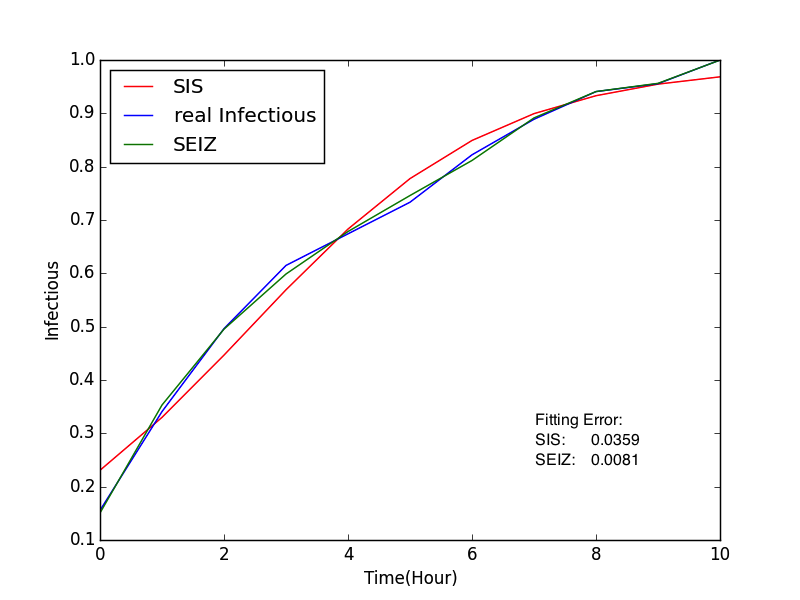
\includegraphics[width=0.48\columnwidth]{images/SISKKKshort.png}
} %
\subfigure[SIS and SEIZ model for rumor 2 with 10 hours data]{\label{fig:SIS-rumor2}
\centering
  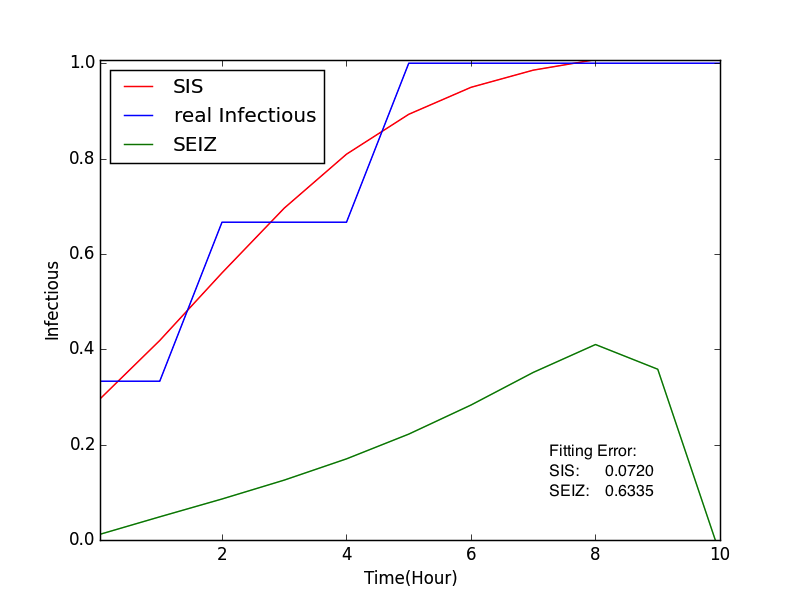
\includegraphics[width=0.48\columnwidth]{images/SIS449short.png}
}
\subfigure[SIS and SEIZ model for news 1 with 10 hours data]{\label{fig:SIS-news1}
\centering
  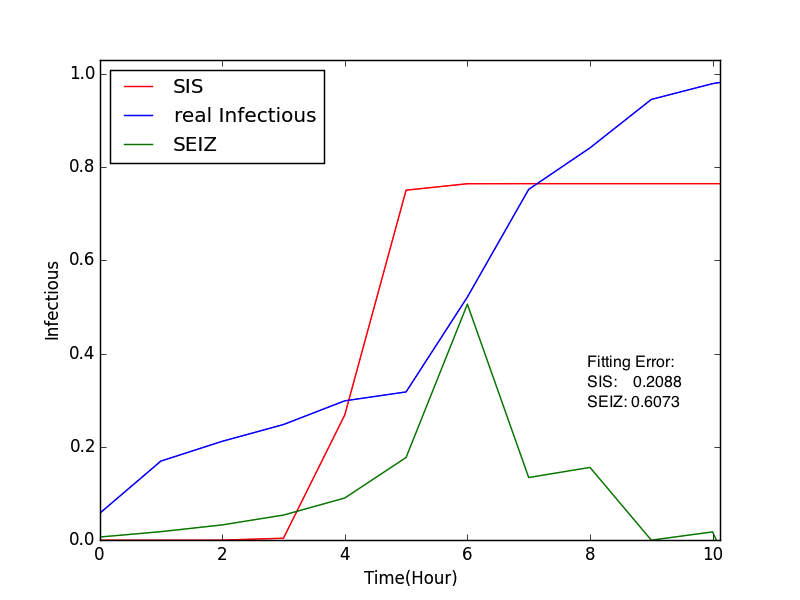
\includegraphics[width=0.48\columnwidth]{images/SISSHUMAshort.png}
}

\subfigure[SIS and SEIZ model for news 2 with 10 hours data]{\label{fig:SIS-news2}
\centering
  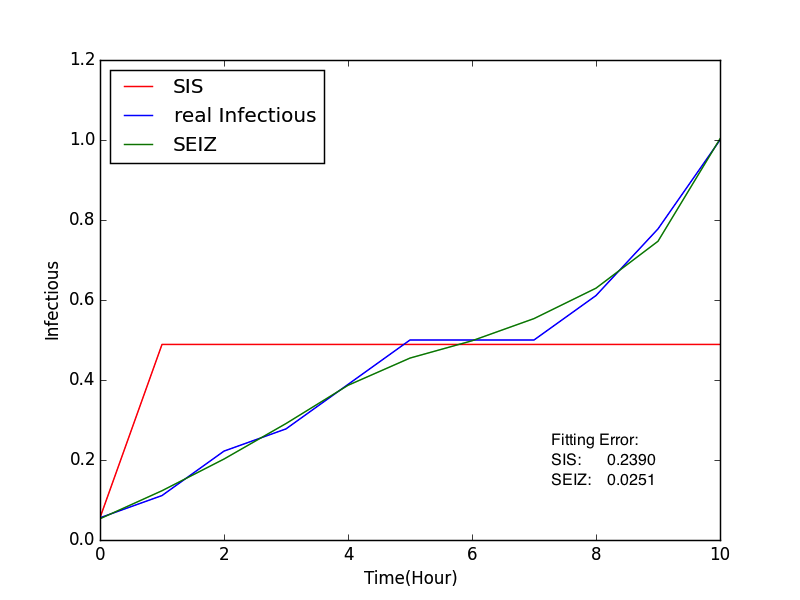
\includegraphics[width=0.48\columnwidth]{images/SIS1347short.png}
}
\caption{Fitting results of SIS and SEIZ model with only first 10 hours tweet volume data (same 4 stories as above)}
\label{fig:SISModelshort}
\end{figure}


\clearpage
\subsection{SpikeM model Features}
Kwon showed us another approach \cite{kwon2013prominent}  for finding the differences between the rumors' propagation pattern and the news events' propagation pattern on twitter. He adjusted the SpikeM Model and also used the parameters as features. 

SpikeM first was introduced by Yasuko Matsubara \cite{conf/kdd/MatsubaraSPLF12} which cab describe the pattern of information diffusion. We present it as follow:

\begin{equation}
\Delta B(n + 1) =p(n + 1)\cdot( U(n) \cdot  \sum ^n_{t=n_b}(\Delta B(t) + S(t))\cdot f(n+1-t) + \varepsilon )
\end{equation}
\begin{equation}
\label{periodic}
p(n) = 1-\frac{1}{2}P_a(\sin (\frac{2\pi}{P_p} (n+P_s)))+1)
\end{equation}

\begin{equation}
U(n + 1)=U(n)-\Delta {B(n + 1) }
\end{equation}
where
\begin{equation}
\label{decay}
f(\tau)=\beta \cdot \tau ^{-1.5}
\end{equation}
and initial conditions:
\begin{equation}
 \Delta B(0)=0 ,U(0) = N
\end{equation}
In addition, adding an external shock $S(n)$, a spike generated
at beginning time $n_b$. Mathematically, it is defined as follows:
\begin{equation}
\label{outs}
S(n) =\begin{cases}0 &(n \neq n_b)\\S_b  & (n =n_b)\end{cases} 
\end{equation}
As the definition: 
\begin{equation}
B(n) + U(n) = N
\end{equation}
The term of $\sum ^n_{t=n_b}(\Delta B(t) + S(t))$ is the total number of informed users at time n, so $\Delta B(n + 1) =p(n + 1)\cdot( U(n) \cdot  \sum ^n_{t=n_b}(\Delta B(t) + S(t))\cdot f(n+1-t) + \varepsilon )$ means that at time n+1 an infected node n randomly select a node m of all nodes and if the node m is susceptible the probability of m turning to infected is $\beta$, so it is a standard SI model. SpikeM extends the SI model from 


 \begin{itemize}
\item a power-law decay term $f(\tau)=\beta \cdot \tau ^{-1.5}
$ in equation \ref{decay}. So the earlier infected nodes has less strength of infection in a power-law decay pattern. 


\item a periodic interaction function in equation \ref{periodic}. It stands for that people have a periodic interaction patterns, like people go to sleep at night so they post much more tweets in the day. Parameters $P_p$, $P_a$, and $P_s$ are the period, strength, and shift of the periodic interaction function.
\item $\varepsilon$ is the background noise term. 
\end{itemize}
\begin{table*}[!h]
 \centering
\scalebox{1}{
\begin{tabular}{@{\textbf{ }}lllllll@{}}
\toprule
\textbf{Symbol} & \textbf{Definition} \\ \midrule
N & total population of available bloggers\\ \midrule
$n_d$	&	duration of sequence\\
n	&	time-tick (n=0, . . . , $n_d$)\\\midrule
U(n)   &	count of \textbf{\underline{u}}n-informed bloggers\\
B(n)   &	count of informed \textbf{\underline{b}}loggers\\
$\Delta B(n)$	&	count of informed \textbf{\underline{b}}loggers at time n\\\midrule
f(n)   &	in\textbf{\underline{f}}ectiveness of a blog-post, at age n\\
$\beta$ & strength of infection\\
$\beta \cdot N$	&	"first-burst" size of infection\\\midrule
S(n)   &	volume of external \textbf{\underline{s}}hock at time n\\
$n_b$ & starting time of \textbf{\underline{b}}reaking news\\
$S_b$	&	strength of external shock at birth (time $n_b$)\\
$\varepsilon$	&	background noise \\\midrule
$P_a$ & strength of periodicity\\
$P_p$			& period of periodicity\\
$P_s$			& phase shift of periodicity\\ \bottomrule

\end{tabular}}
\caption{Parameters of SpikeM}
\label{tab:Features_Impsortance}
\end{table*}
But the SpikeM can't fit to the events with multi-pike like the figure \ref{fig:KKK_part}. So the author think the term external shock $S(n)$ in equation \ref{outs} should not occur once but more. So they extend the SpikeM model by adding a periodic interaction function the term external shock $S(n)$.

\begin{equation}
\Delta B(n + 1) =p(n + 1)\cdot( U(n) \cdot  \sum ^n_{t=n_b}(\Delta B(t) +  \bar{S}(t))\cdot f(n+1-t) + \varepsilon )
\end{equation}
\begin{equation}
\label{periodic}
p(n) = 1-\frac{1}{2}P_a(\sin (\frac{2\pi}{P_p} (n+P_s)))+1)
\end{equation}

\begin{equation}
U(n + 1)=U(n)-\Delta {B(n + 1) }
\end{equation}
\begin{equation}
\label{decay}
f(\tau)=\beta \cdot \tau ^{-1.5}
\end{equation}
The external shock $S(n)$ is added a a periodic interaction function
\begin{equation}
\label{outs}
\bar{S}(t)=S(t)+q(t)
\end{equation}
\begin{equation}
q(t) =  q_a(\sin (\frac{2\pi}{q_p} (t+q_s)))+1)
\end{equation}


\begin{table*}[!h]
 \centering
\scalebox{1}{
\begin{tabular}{@{\textbf{ }}lllllll@{}}
\toprule
\textbf{Symbol} & \textbf{Definition} \\ \midrule
$q_a$ & strength of periodicity of the external shock\\
$q_p$			& period of periodicity of the external shock\\
$q_s$			& phase shift of periodicity of the external shock\\ \bottomrule

\end{tabular}}
\caption{New Parameters of extended SpikeM}
\label{tab:Features_Impsortance2}
\end{table*}
As the same approach of fitting SIS model, we learn the parameters of SpikeM model with Levenberg-Marquard algorithm. We fit the sequenced tweet volume from the beginning time the $t_0$ to the current time interval $t_n$ of an event to the model and use the output parameters as the features adding into DSTS. We use the $p_a$,  $p_p$, $p_s$ and $q_a$, $q_p$, $q_s$ as feature. We show 4 examples of the SpikeM fitting result in figure \ref{fig:SPikeModel}. But same problem as fitting SIS or SEIZ, if we test only within 10 hours data the result seems much worse than the result with full 48 hours showing in figure \ref{fig:SpikeMModelshort}.

\begin{figure}[!h]

  \centering

\subfigure[SIS and SEIZ model for rumor 1]{\label{fig:SPikeM-rumor1}
\centering
  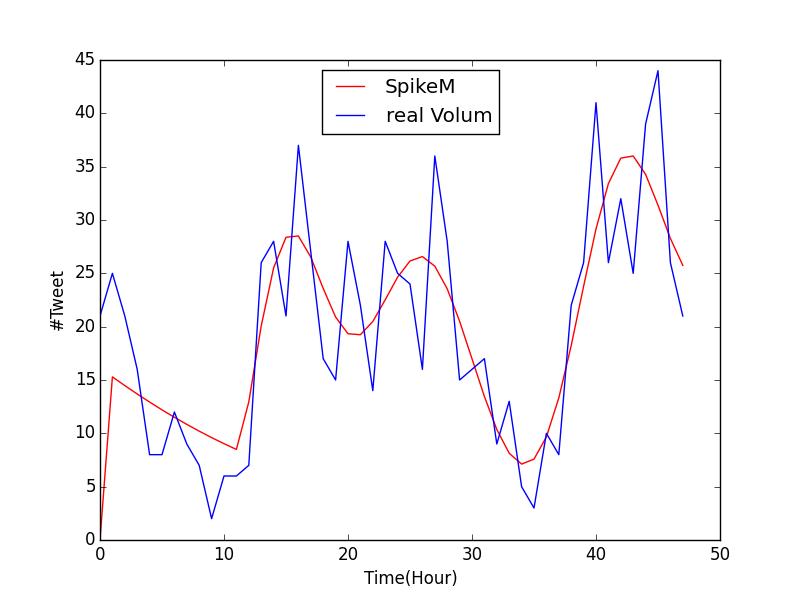
\includegraphics[width=0.48\columnwidth]{images/SpikeM_kkk.png}
} %
\subfigure[SIS and SEIZ model for rumor 2 ]{\label{fig:SPikeM-rumor2}
\centering
  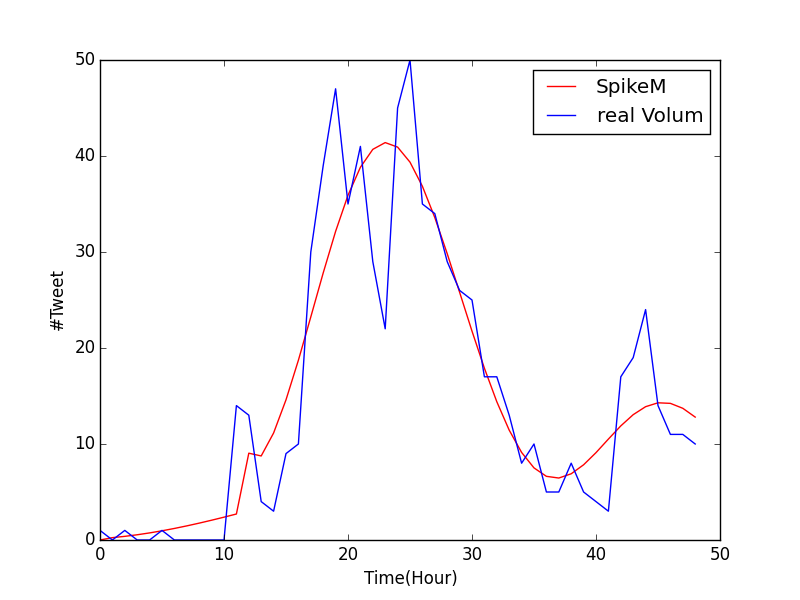
\includegraphics[width=0.48\columnwidth]{images/SpikeM_449.png}
}
\subfigure[SIS and SEIZ model for news 1]{\label{fig:SPikeM-news1}
   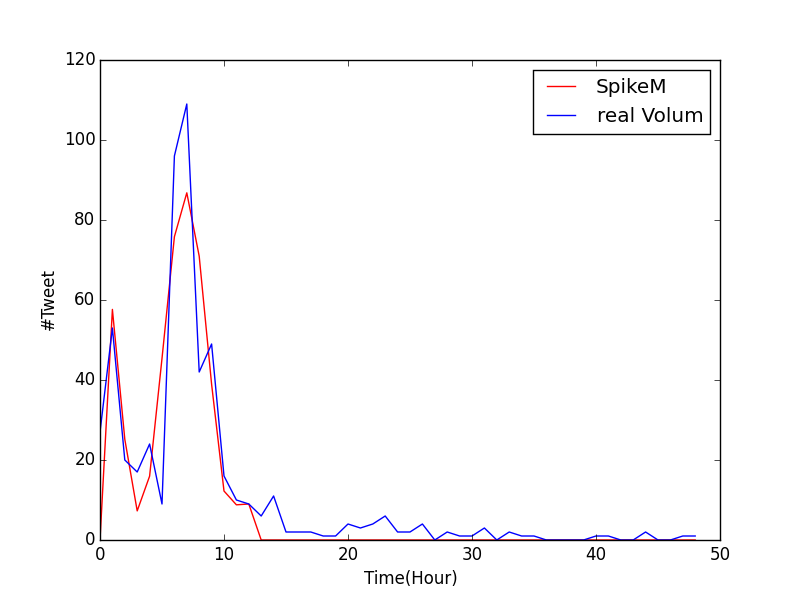
\includegraphics[width=0.48\columnwidth]{images/SpikeMSchuma.png}
}

\subfigure[SIS and SEIZ model for news 2 ]{\label{fig:SPikeM-news2}
   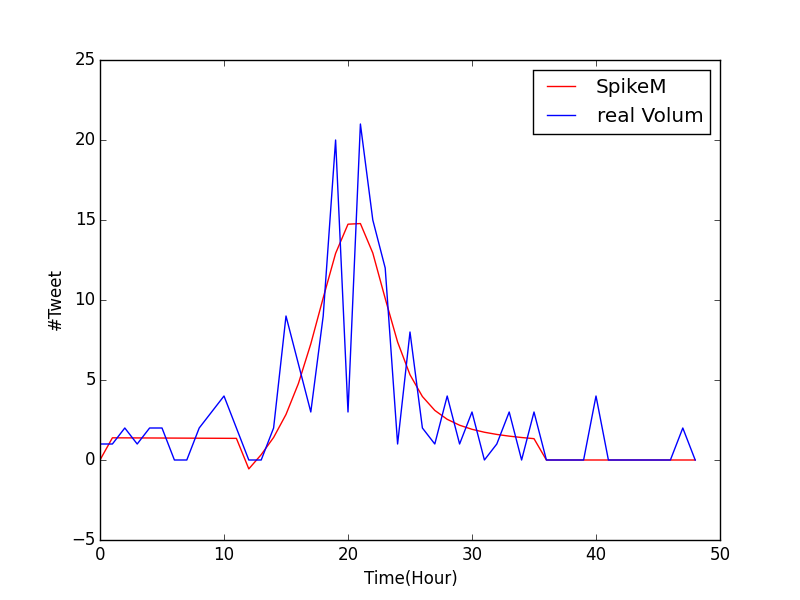
\includegraphics[width=0.48\columnwidth]{images/SpikeM_1347.png}
}
\caption{Fitting results of SpikeM model of (a) Rumor: Robert Byrd was a member of KKK (b) Rumor: CNN altered a photograph of a shooter making him look white (c) News: Doctor announces Michael Schumacher is making process (d) News: Two U.S. sailors are arrested over an alleged rape of a Japanese woman on Okinawa }
\label{fig:SPikeModel}
\end{figure}

\begin{figure}[!h]

  \centering

\subfigure[SIS and SEIZ model for rumor 1 with 10 hours data]{\label{fig:SPikeM-rumor1}
\centering
  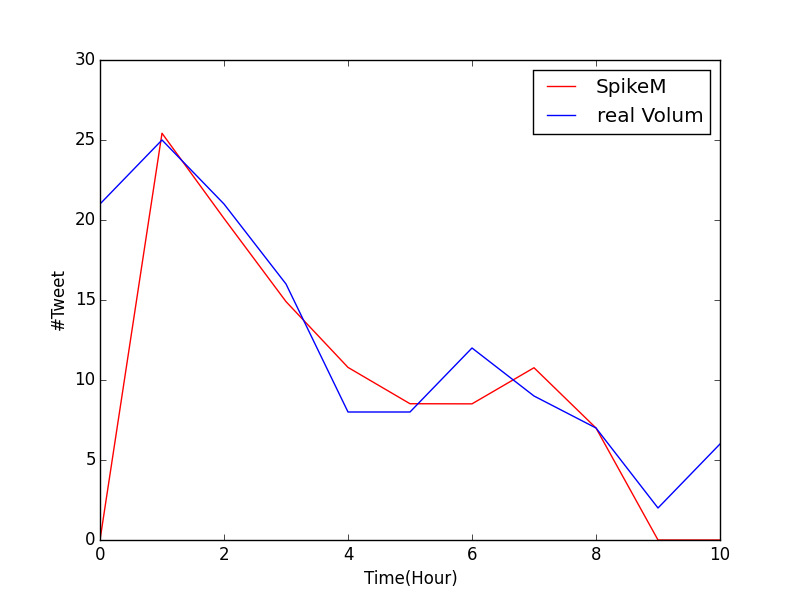
\includegraphics[width=0.48\columnwidth]{images/SpikeMKKKshort.png}
} %
\subfigure[SIS and SEIZ model for rumor 2 with 10 hours data]{\label{fig:SPikeM-rumor2}
\centering
  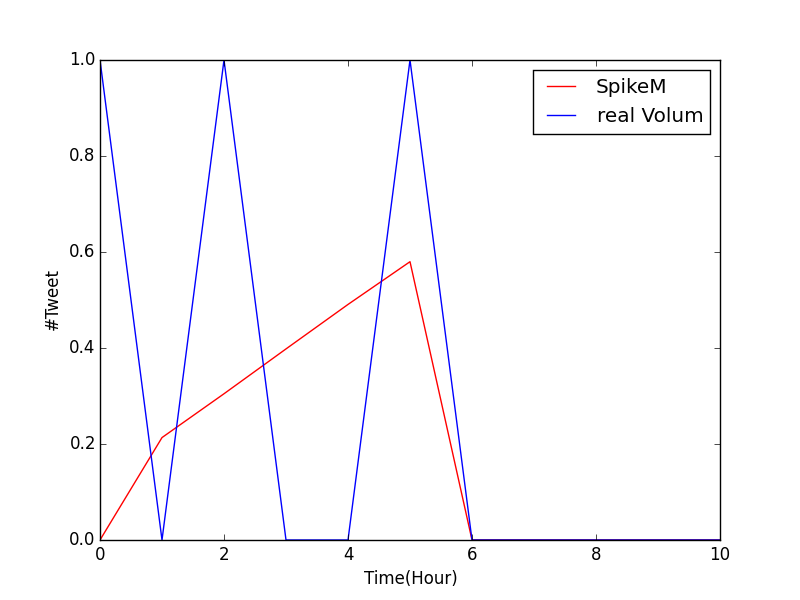
\includegraphics[width=0.48\columnwidth]{images/SpikeM492short.png}
}
\subfigure[SIS and SEIZ model for news 1 with 10 hours data]{\label{fig:SPikeM-news1}
\centering
  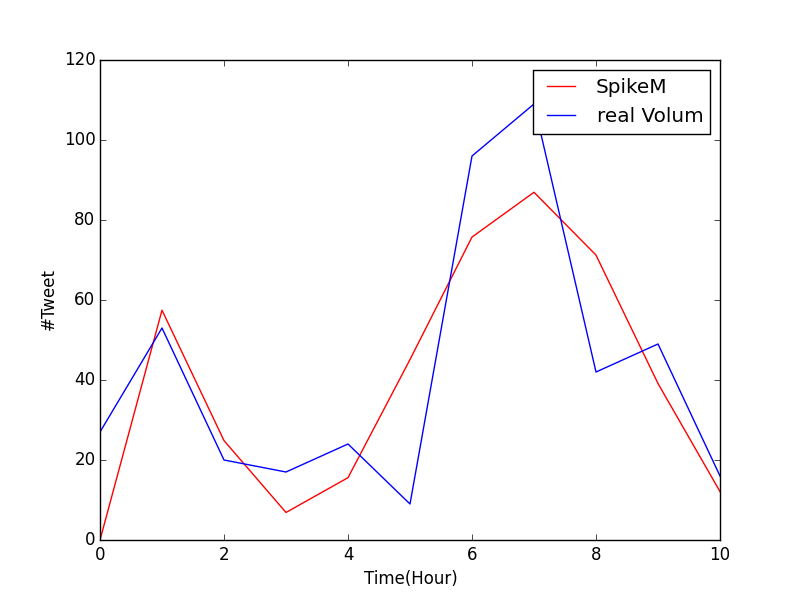
\includegraphics[width=0.48\columnwidth]{images/SpikeMSHUshort.png}
}

\subfigure[SIS and SEIZ model for news 2 with 10 hours data]{\label{fig:SPikeM-news2}
\centering
  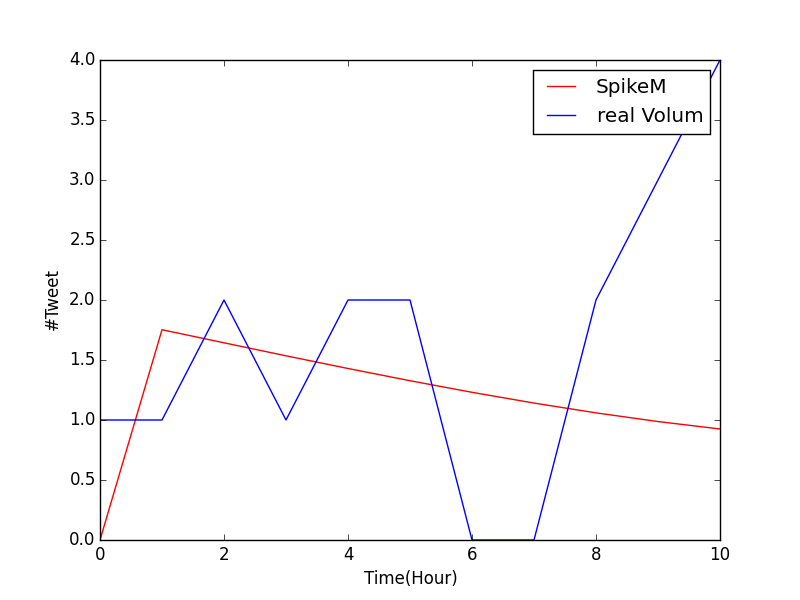
\includegraphics[width=0.48\columnwidth]{images/SpikeM1347short.png}
}
\caption{Fitting results of SpikeM model with first 10 hours data (same stories as above) }
\label{fig:SpikeMModelshort}
\end{figure}

\clearpage
\subsection{Crowd Wisdom Features}
The idea come from Liu's work \cite{liu2015real} but not same. The core idea is using the public's common sense to detecting the rumors. If there are more people denying or doubting the truth of an event, this event are more likely to be a rumor. 
In the Liu's work he uses a extensive list of positive, negative and negation keywords and a set of rules like "negative words without negation words means the poster denies the event". And he uses the ratio  number of positive  poster (supporter) to the negative poster (deny the events).

Our work is simpler than than his work. We have only a set of negative words, we call it "debunking words" like hoax, rumor, not true, etc.  In our test, it is a good feature, but it needs 17 hours to "warm up". It is logical because crowds can debunk rumors but they need time to wait the professionals' advices or to unify the attitude the event.

\subsection{CreditScore Features}
This feature is new feature. We our trained single tweet's creditability model the predict the tweets of the events. If the output is rumor we label it 1 otherwise 0 and we calculate the average score of the events in certain hour. We call this feature creditsScore. We will show it late, this is the best of our dataset, it improves the  performance of time series model especially in the first 12 hours. When the event begin bursting in the early stage, people can only rely on the information from the single tweet itself. Because there is no clear propagation structure (pattern) or the wise men or journalists deny the event yet. Our neural network model "sees and check" the text of a single tweet and "give us the advise" when we have no other features in the first few hours since the beginning of the events. 

The result shows this feature is the best feature.
 
\clearpage
\begin{table*}[!h]
\small
\centering
\scalebox{0.8}{
 \begin{tabular}{@{}lllllll@{}}
 \toprule
 \textbf{Category} & \textbf{Feature} & \textbf{Description}\\ \midrule
 Twitter Features& Hashtag & \% of the tweets containing \#hashtag  \cite{castillo2011information}\cite{liu2015real}\cite{qazvinian2011rumor}\cite{gupta2014tweetcred}\cite{liu2015real}\\
 		& Mention &  \% of the tweets mentioning others @user  \cite{castillo2011information}\cite{liu2015real}\cite{qazvinian2011rumor}\cite{gupta2014tweetcred}\cite{liu2015real}\\
 		& NumUrls &  \# of url in the tweet  \cite{castillo2011information}\cite{qazvinian2011rumor}\cite{gupta2014tweetcred}\cite{yang2012automatic}\cite{liu2015real}\\
 		& Retweets & average times of tweets have been retweeted \cite{liu2015real} \\ 
 		& IsRetweet & \% of tweets are retweeted from others \cite{castillo2011information}\cite{gupta2014tweetcred}\\
 		& ContainNEWS & \% of tweets containing URL and its domain's catalogue is News \cite{liu2015real}\\
 		& WotScore & average WOT score of domain in URL \cite{gupta2014tweetcred}\\
 		& URLRank5000 & \% of tweets contains URL whose domain's rank less than 5000 \cite{castillo2011information}\\
 		& ContainNewsURL & \% of tweets contains URL whose domain is News Website\\
\midrule
 Text Features & LengthofTweet & average length of tweets  \cite{castillo2011information}\cite{gupta2014tweetcred}\\
    & NumOfChar & average number of individual characters of tweets \cite{castillo2011information}\cite{gupta2014tweetcred}\\
   & Capital &  average fraction of characters in Uppercase of tweets \cite{castillo2011information} \\
   & Smile & \% of tweets containing :->, :-), ;->, ;-) \cite{castillo2011information}\cite{gupta2014tweetcred}\\
   & Sad & \% of tweets containing :-<, :-(, ;->, ;-( \cite{castillo2011information}\cite{gupta2014tweetcred}\\
   & NumPositiveWords & average number of positive words \cite{castillo2011information}\cite{gupta2014tweetcred}\cite{yang2012automatic}\cite{liu2015real}\\
   & NumNegativeWords & average number of negative words \cite{castillo2011information}\cite{gupta2014tweetcred}\cite{yang2012automatic}\cite{liu2015real}\\
   & PolarityScores & average polarity scores of the Tweets \cite{castillo2011information}\cite{yang2012automatic}\cite{liu2015real}\\
   & Via & \% of tweets containing via \cite{gupta2014tweetcred}\\
   & Stock & \% of tweets containing \$  \cite{castillo2011information}\cite{gupta2014tweetcred}\\
   & Question & \% of tweets containing ? \cite{castillo2011information}\cite{liu2015real}\\
   & Exclamation & \% of tweets containing ! \cite{castillo2011information}\cite{liu2015real}\\
   & QuestionExclamation & \% of tweets containing multi Question or Exclamation mark \cite{castillo2011information}\cite{liu2015real}\\ 
   & I & \% of tweets containing first pronoun like I, my, mine, we, our    \cite{castillo2011information}\cite{gupta2014tweetcred}\cite{liu2015real}\\
   & You & \% of tweets containing second pronoun like U, you, your, yours  \cite{castillo2011information}\\ 
   & HeShe & \% of tweets containing third pronoun like he, she, they, his, etc.  \cite{castillo2011information}\\ \midrule
   User Features & UserNumFollowers  & average number of followers \cite{castillo2011information}\cite{gupta2014tweetcred}\cite{liu2015real}\\
 	& UserNumFriends  & average number of friends \cite{castillo2011information}\cite{gupta2014tweetcred}\cite{liu2015real}\\
 	& UserNumTweets  & average number of users posted tweets \cite{castillo2011information}\cite{gupta2014tweetcred}\cite{yang2012automatic}\cite{liu2015real}
\\
 	& UserNumPhotos  & average number of users posted photos \cite{yang2012automatic}\\
 	& UserIsInLargeCity  & \% of users living in large city \cite{yang2012automatic}\cite{liu2015real}\\
 	& UserJoinDate & average days since users joining Twitter \cite{castillo2011information}\cite{yang2012automatic}\cite{liu2015real}
\\
 	& UserDescription  & \% of user having description \cite{castillo2011information}\cite{yang2012automatic}\cite{liu2015real}
\\
 	& UserVerified  & \% of user being a verified user\cite{yang2012automatic}\cite{liu2015real}
\\
 	& UserReputationScore & average ratio of \#Friends over (\#Followers + \#Friends) \cite{liu2015real}\\   \midrule
 Epidemiological Features & $\beta_{SIS}$ & Parameter $\beta$ of Model SIS \cite{jin2013epidemiological}\\
 							& $\alpha_{SIS} $ & Parameter $\alpha$ of Model SIS \cite{jin2013epidemiological}\\
 							& $\beta_{SEIZ}$ & Parameter $\beta$ of Model SEIZ \cite{jin2013epidemiological}\\
 							& $b_{SEIZ}$ & Parameter b of Model SEIZ\cite{jin2013epidemiological}\\
 							& $l_{SEIZ}$ & Parameter l of Model SEIZ \cite{jin2013epidemiological}\\
 							& $p_{SEIZ}$ & Parameter p of Model SEIZ \cite{jin2013epidemiological}\\
 							& $\varepsilon_{SEIZ}$ & Parameter $\varepsilon$ of Model SEIZ \cite{jin2013epidemiological}\\
 							& $\rho_{SEIZ}$ & Parameter $\rho$ of Model SEIZ \cite{jin2013epidemiological}\\
 							& $R_{SI}$ & Parameter $R_{SI}$ of Model SEIZ \cite{jin2013epidemiological}\\
		\midrule	
 SpikeM Model Features & $P_s$ & Parameter $P_s$ of Model Spike \cite{kwon2013prominent}\\
 							& $P_a$ & Parameter $P_a$ of Model SpikeM \cite{kwon2013prominent}\\
 							& $P_p$ & Parameter $P_p$ of Model SpikeM \cite{kwon2013prominent}\\
 							& $Q_s$  & Parameter $Q_s$ of Model SpikeM \cite{kwon2013prominent}\\
 							& $Q_a$ & Parameter $Q_a$ of Model SpikeM \cite{kwon2013prominent}\\
 							& $Q_p$ & Parameter $Q_p$ of Model SpikeM \cite{kwon2013prominent}\\ \midrule	
 Crowd Wisdom Features & CrowdWisdom & \% of tweets containing "Debunking Words" \cite{liu2015real} \cite{zhao2015enquiring}\\ \midrule
 Credit Score Features & CreditScore & average CreditScore\\
 \bottomrule
 \end{tabular}}
 \caption{Features of Time Series Rumor Detection Model}
 \label{tab:full_features}
\end{table*}
\clearpage
  \section{ Classification Models } 
Same reason as the single tweet's Creditability we test the time series model also with 3 popular models Decision Trees, SVM,  Random Forest and one more model the multilayer perceptron (MLP). We show the optimized parameters in the table \ref{tab:time_model_para}. After 10-fold cross validation with same shuffled sequence  testing above models, the result is shown the figure \ref{tab:time_result}.  

\begin{table*}[!h]
 \centering
\scalebox{0.8}{
 \begin{tabular}{@{}l|l|l@{}}
 \toprule
 \multicolumn{1}{l|}{\textbf{Model}} &\multicolumn{1}{l|}{ \textbf{Parameters} }& \textbf{Value} \\ \midrule
 $Random Forest_{ts}$ & Number of Trees & 350\\ \midrule
 $SVM_{DSTS}$\cite{ma2015detect} & kernel  & radial basis function\\
 	& penalty parameter of the error term  & 3.0\\
 	& gamma  & $\frac{1}{50}$\\ \midrule
 Decision Trees & criterion & gini \\ \midrule
  MLP & alpha  & 0.0001\\
 	& activation function  & ReLU\\
 	& hidden layer sizes  & 2 layer(50 nodes each layer)\\
 	&weight optimization & adam\\ 
 \bottomrule
 \end{tabular}}
 \caption{Parameters of Classification models}
 \label{tab:time_model_para}
\end{table*}


\clearpage
  \section{Experiment Setting } 
\label{cha:Data_Collection}
We collected rumor stories from a rumor tracking website \textbf{snopes.com} and \textbf{urbanlegends.about.com}. We crawled 4300 stories from the website and we manually constructed 130 queries of them. The approach of constructing queries is mainly following the work\cite{gupta2014tweetcred}. The regular expression of a query is:

$(Object \& Subject \& Description(Description1||Description2||...))$


for example a story is about Obama removing a flag in pearl harbor. Object is Obama, subject is flag and its synonym like flags, flagpole. Description is remove and its synonym removes, removed, removal, removing, "token down" or a url about this rumor "Departed.co". In this case there is a proper noun "pearl harbor" is also useful. Finally we transfer the regex to Twitter's query: Obama (flag OR flags OR flagpole) (remove OR removes OR removed OR removal OR removing OR "token down" OR "Departed.co") pearl harbor.


%to do %
Pervious work \cite{liu2015real} used the news which are reported on snopes.com. But after we test them, we think these news event contain too less tweets. So we use the dataset from the work of Mcminn et al.\cite{mcminn2013building}. These events are manually checked that they really happened. We pick the top 90 events contains most tweet volume and we add other 40 famous news events like Munich shooting.

The detail of tweet volume is shown in table \ref{tab:Tweet_Volume}.

After we crawled and parsed the whole timeline of an event. We detect the 48 hours time period of the burst in the way we mentioned in section \ref{sec:Time_Period_of_an_Event}. We crawled the homepage of poster of the tweets within the event time period total 133,396 users. We also extracted 11,038 domains which are contained in the tweets in the 48 hours time period and we crawled these domains' catalogs in bluecoat.com \footnote{http://sitereview.bluecoat.com/sitereview.jsp\#/?search=bbc.com}, their ranks in alexa.com\footnote{http://www.alexa.com/siteinfo/bbc.com} and WOT score in wot.com \footnote{https://www.mywot.com/en/api}. 

As we told in the section \ref{tapi}, the Twitter limits its API with the return result only in recent 7 days. So we have to crawl the data from the web interface. We use Beautiful Soup as the html parsing library to parse the Twitter timeline pages and the users' homepage \footnote{https://www.crummy.com/software/BeautifulSoup/bs4/doc/}. Beautiful Soup is a Python library for pulling data out of HTML and XML files. For increasing the speed of parsing html and extracting features from raw data, we use Spark\footnote{http://spark.apache.org/} technology, because it can simply manage multithread and its mapReduce in memory technology makes the process much faster. 
 
\begin{table*}[!h]
 \centering
\scalebox{0.8}{
 \begin{tabular}{@{}cccccc@{}}
 \toprule
 \textbf{Type} & \textbf{Min Tweet Volume} & \textbf{Max Tweet Volume}& \textbf{Total Tweet Number} &\textbf{Average Tweet Number} \\ \midrule
 News & 18 & 17414 & 172616 & 1327.82 \\ \midrule
 Rumors & 44  & 26010& 91268 & 702.06\\
 	 \bottomrule
 \end{tabular}}
 \caption{Tweet Volume of News and Rumors}
 \label{tab:Tweet_Volume}
\end{table*}
\clearpage
  \section{Experiment Result } 
  
  The $Random Forest_{ts}$ is the best model for our task, so we use RF as the test model for the further features' Evolution.
\begin{table}[]
\centering
\begin{tabular}{|c|cccc|}
\hline
\multicolumn{1}{|c|}{\multirow{2}{*}{Model}} & \multicolumn{4}{c|}{Accuracy in hours}                     \\ \cline{2-5} 
\multicolumn{1}{|l|}{}& 6 & 12 & 24 & \multicolumn{1}{c|}{48} \\\hline
 $Random Forest_{ts}$  & \textbf{0.8615} &  \textbf{0.8615}  &\textbf{ 0.8692} &  \textbf{0.9076 }\\
$MLP_{DSTS}$ & 0.7423  & 0.7423   &   0.7692   &  0.8192 \\
$SVM_{DSTS}$\cite{ma2015detect} & 0.7423  & 0.7884   &   0.7769   & 0.7538  \\
$DT_{DSTS}$\cite{ma2015detect}& 0.7807  & 0.8115   &  0.75 & 0.7385 \\    \bottomrule           
\end{tabular}
 \caption{Prediction Accuracy of Different Single Tweet's Creditability Scoring Models}
 \label{tab:time_result}
\end{table}

    \subsection{$Random Forest_{ts}$ VS Static Features} 

First we compare our time series model and the normal static feature model. We show the result is in table \ref{TVSF} the full 48 hours details in Appendix table \ref{TSVSSFFULL} and in figure \ref{fig:TVSF}. As we can see from the result that the accuracy of time Series in most of time is better than the static model. But after 24 hours the advantage of the time series is very limited. The reason may be after 24 hours the static model already has enough data to ignore the offset of features at the different time points. But the time series model still has the benefit of detecting rumors at the beginning of spreading. 
 
\begin{table}[!h]
\centering
\begin{tabular}{|c|c c |c|}
\hline
Hour & $Random Forest_{ts}$ & Static model & Difference \\ \hline
1    & 0.82              & 0.78         & 0.03       \\
6    & 0.86              & 0.8          & 0.06       \\
12   & 0.87              & 0.83         & 0.04       \\
18   & 0.88              & 0.83         & 0.05       \\
24   & 0.87              & 0.85         & 0.01       \\
30   & 0.88              & 0.85         & 0.03       \\
36   & 0.87              & 0.86         & 0.01          \\
42   & 0.88              & 0.88         & 0          \\
48   & 0.89              & 0.87         & 0.02      \\\hline

\end{tabular}
\caption{Accuracy: Time Series VS Static Features}
\label{TVSF}
\end{table}

\begin{figure}[!h]
\centering
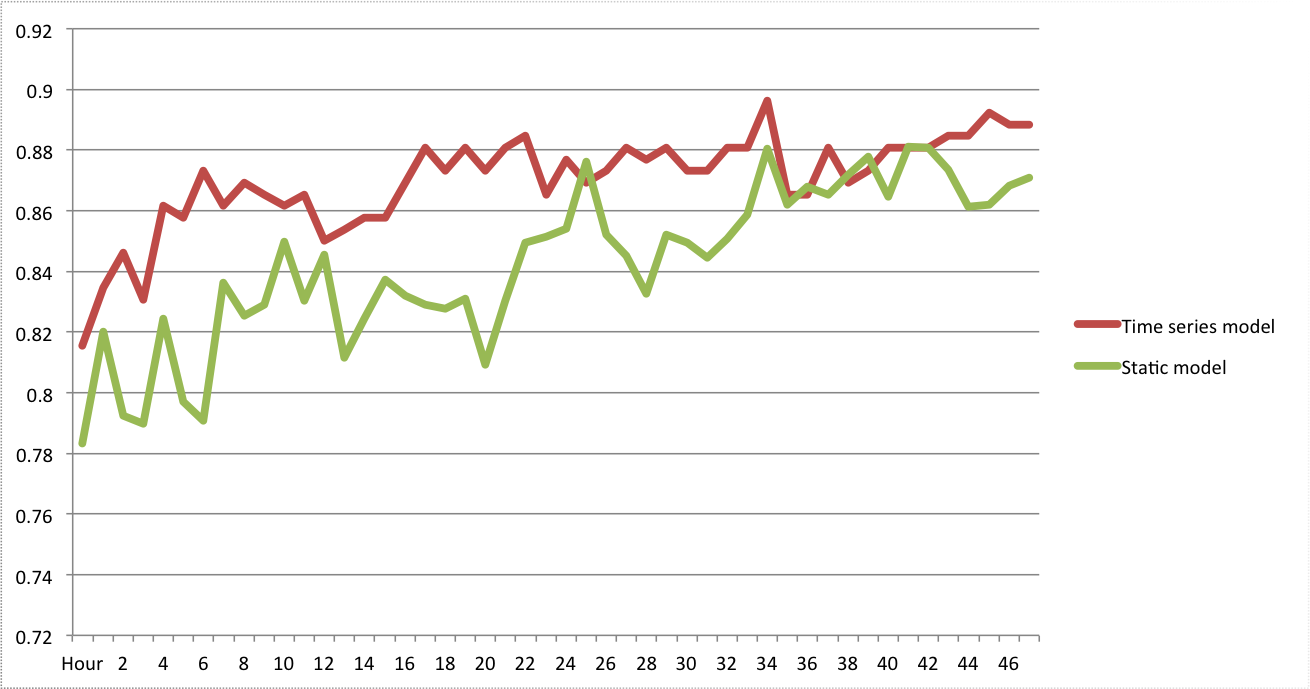
\includegraphics[width=0.8\columnwidth]{images/Vsstatic.png}
\caption{Accuracy: Time Series VS Static Features}
\label{fig:TVSF}
\end{figure}

  \newpage
 \subsection{Feature Analyzing Over Time} 
 \label{featureanalyzing}
 We rank the features' importance using the method we introduced in section \ref{random_forest}, the full result is shown in appendix table \ref{tab:allfeaturerank}.  First we split the features in 7 catalogues as in table \ref{tab:full_features}: Tweet\_Feature, User\_Feature,Text\_Feature,  Credit Score, SpikeM Features, Epidemiological Features, CrowdWisdom and the BestSet. The BestSet is a combination of the 28 top best average rank of 48 hours features, they are shown in table \ref{bestfeature}. The results over 48 hours are in figure \ref{fig:allfeature} .
 
 \begin{table}[!h]
\centering
\begin{tabular}{l|l}
\hline

\multicolumn{2}{c}{Best Feature set} \\\hline

 CreditScore & ContainNEWS \\

NumOfChar  & UserTweetsPerDays\\
QuestionExclamation  & UserReputationScore\\ 
 
WotScore  & Question\\
UserJoin\_date  & Mention\\
LengthOfTweet  & DebunkingWords\\
UserFollowers  & Exclamation\\
UserVerified  &  Hashtag\\

Capital   & You\\
UserNumPhoto   & numUrls\\
UserFriends   & NumPositiveWords\\
Via   & $P_a$\\

UserIsInLargeCity  & PolarityScores \\UserDescription  & $R_{SI}$  \\ \bottomrule 
 \end{tabular}
\caption{Best Features}
\label{bestfeature}
\end{table}

 \begin{figure}[!h]
\centering
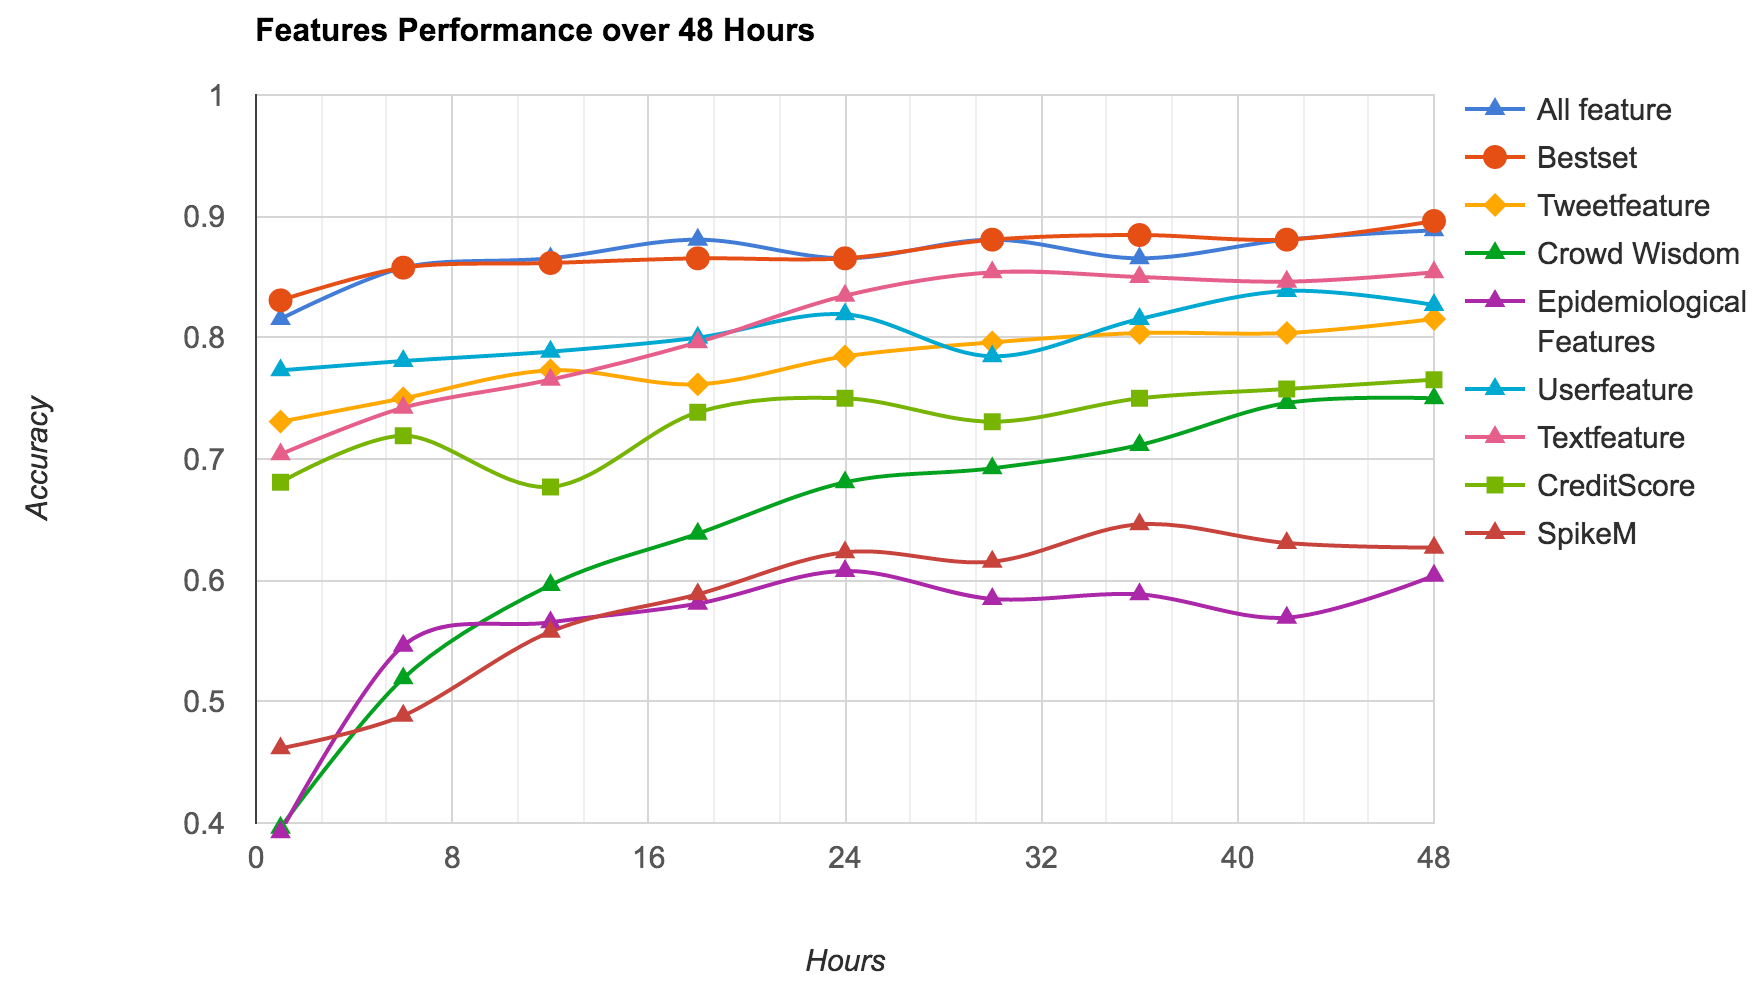
\includegraphics[width=\columnwidth]{images/allfeatures.png}
\caption{Accuracy: Time series VS static Features}
\label{fig:allfeature}
\end{figure}
 
 As we can see in figure \ref{fig:allfeature} the best result on average over 48 hours in the \emph{BestSet} with top 28 features. Second is the  \emph{All features}. Except those two the best group feature is \emph{Text feature}. One reason is the text feature set has the largest group of feature with totally 16 features. But if look into each feature in text feature group we can see the best and the worst features are all in this set. \emph{User feature} and \emph{Twitter feature} are stable over time around 82\%. The performances of 3 different models (SIS, SEIZ and SpikeM) describing the propagation pattern of rumors and news are not so well especially within 24 hours. \emph{Crowd Wisdom} and \emph{Credit Score} both contain only one feature but they already have impressive result comparing with the \emph{User feature} and \emph{Twitter feature}.
 \subsection{BestSet Features} 
 We pick the 28 top best average rank of 48 hours features, see table \ref{bestfeature} and group them as the BestSet Feature. Adding one more feature and removing one will both cause the accuracy dropping down. So we think it is the best combination of features for rumor detection.
 
 \subsection{Text Features} 
 \emph{Text feature} set contains 16 features. The ranks of feature as shown in table \ref{testfeaturerank}. The best one is \emph{NumOfChar} which is the average number of different characters in tweets. It is quite hard to explain why it is like that. 
 
 \emph{PolarityScores} is the best feature when we tested the single tweets model, but its rank in time series model is not so good.  It is true that rumor contains more negative sentiment, but in an event (rumor or news) people can show their different views about this event \cite{mendoza2010twitter} \cite{starbird2014rumors} like discussing or denying, so the \emph{ PolarityScores}'s performance becomes worse and worse over time. 
  \emph{Text feature} overall is the the best feature set.
 
 \begin{table}[!h]
 \centering
\scalebox{1}{
\begin{tabular}{@{\textbf{ }}ccccccccccccccccc@{}}
\toprule
\textbf{Features} & \multicolumn{10}{c}{\textbf{Ranks}} \\\hline
Hours & 1 & 6 & 12 & 18&24&30&36&42&48 & AVG\\\hline
 %ContainNEWS & 8 & 4 & 5& 4 & 4&2&2&2&2&3.48\\
NumOfChar			& 3& 3 & 4 & 3& 3& 8& 7&6 & 4& 4.29\\
QuestionExclamation		& 25& 16 & 2 & 1& 1& 1& 3& 7&5&4.79\\
%UrlRankIn5000			& 14& 13 & 7 & 11 & 7& 3& 1& 4&6&4.79\\
%WotScore			& 4 & 10& 6 & 10 & 10& 6& 9& 8&7&7.63\\ 
Question 			& 15 & 11& 13 & 7 & 5& 4& 8& 5&8&8.29\\ 
%Mention 			& 13 & 5& 10 & 14 & 13& 10& 12& 12&10&10.98\\
LengthOfTweet 			& 6 & 6& 9 & 6 & 14& 16& 13& 16&13&11.96\\ 
PolarityScores & 12 & 15& 23 & 28 & 33& 33& 34& 31&32&28\\

Stock 			& 34 & 44& 47 & 47 & 47& 47& 47& 47&48&46.15\\ 
Smile 			& 35 & 45& 45 & 48 & 48& 48& 48& 48&48&47.06\\ 
 
Sad 			& 36 & 46& 46 & 49 & 49& 49& 49& 49&49&47.9\\ 

\bottomrule
 \end{tabular}}
\caption{Rank of Part of Text Feature}
\label{testfeaturerank}
\end{table}
 \subsection{Twitter Features} 
   \emph{Twitter feature} is stable over time from the beginning to the end.

 The 3 best of \emph{Tweet Features} are all the features about the contained ULR in tweet: \emph{ContainNEWS}, \emph{UrlRankIn5000}, \emph{WotScore} showing in table \ref{twitterfeaturerank}. It it quite logical that the news will have higher probability reported by news websites or higher ranked website. And it is clear to see the that their performance significantly improve after 24 hours.
 

 But the other original twitter functions like the retweets or mention do not contribute much.
 

\begin{table}[!h]
\centering
\scalebox{1}{
\begin{tabular}{@{\textbf{ }}ccccccccccccccccc@{}}
\toprule
\textbf{Features} & \multicolumn{10}{c}{\textbf{Ranks}} \\\hline
Hours & 1 & 6 & 12 & 18&24&30&36&42&48 & AVG\\\hline
ContainNEWS & 8 & 4 & 5& 4 & 4&2&2&2&2&3.48\\
UrlRankIn5000			& 14& 13 & 7 & 11 & 7& 3& 1& 4&6&5.96\\
WotScore			& 4 & 10& 6 & 10 & 10& 6& 9& 8&7&7.63\\ 
%Question 			& 15 & 11& 13 & 7 & 5& 4& 8& 5&8&8.29\\ 
Mention 			& 13 & 5& 10 & 14 & 13& 10& 12& 12&10&10.98\\
Hashtag 			& 20 & 20& 15 & 18 & 16& 13& 15& 17&17&17.46\\ 
Retweets & 21 & 21& 27 & 38 & 42& 35& 31& 37&34&33.25\\
\bottomrule
 \end{tabular}}
\caption{Rank of Part of Twitter Feature}
\label{twitterfeaturerank}
\end{table}

\subsection{User Features} 
The performance of user features is similar with the twitter, they are both quite stable from the first hour to the last hour. But one difference is in the first few user feature is the best feature set except all feature set.

As in table \ref{userfeaturerank} shown, the best feature of user feature is UserTweetsPerDays. And it is the best feature overall in the first 4 hours, but it drops down over time. Others user features like Reputation Score and Join date have also better performance at the first fews hours. 

That means the sources (the poster in the first few hours) of news and rumors are quite different with each other, but more and more users join in the discussion, so the bias of two groups of user is less and less. After 6 hours we distinguish the rumors basing on the content of the tweet(text features) already better basing on the feature of the poster.
 
\begin{table}[!h]
\centering
\scalebox{1}{
\begin{tabular}{@{\textbf{ }}ccccccccccccccccc@{}}
\toprule
\textbf{Features} & \multicolumn{10}{c}{\textbf{Ranks}} \\\hline
Hours & 1 & 6 & 12 & 18&24&30&36&42&48 & AVG\\\hline
UserTweetsPerDays & 0 & 1 & 1& 2 & 2&9&5&10&14&4.63\\
UserReputationScore	 & 1& 2 & 3 & 5 &6& 5& 6& 3&3&5.06\\
UserJoin\_date			& 5 & 8& 8 & 8 & 12& 14& 16& 11&9&10.58\\ 
UserVerified 			& 24 & 17& 12 & 16 & 17& 12& 11&14&19&16.25\\ 
 \bottomrule
 \end{tabular}}
\caption{Rank of Part of User Feature}
\label{userfeaturerank}
\end{table}
\subsection{SpikeM Features and Epidemiological Features}
The two feature sets of these two models seem not so well. 
Only one feature $P_a$ from the SpikeM is added in the BestSet features. 
As the problem of these two models which we have already figured out in section \ref{sec:epide} is Both of these models need enough data to fit the parameters. Only after 24 hours these two models' features can reach 60\% accuracy. In other words before 24 hour these is no clear propagation pattern of these events. In the work of Kwon \cite{kwon2013prominent}, the durations of dataset which he uses are more than (wenxian). In the work of Jin\cite{jin2013epidemiological}, he uses () to fit the SEIZ models. Their data's durations are far larger than ours 48 hours.
 
 $P_a$ parameter from SpikeM is the only one feature in the top 26 feature set. It stands for the strength of periodicity.  Kwon add 3 more parameters to explain the periodicity of the external shock. They are not so functional because of short time period.

\begin{table}[!h]
\centering
\scalebox{1}{
\begin{tabular}{@{\textbf{ }}ccccccccccccccccc@{}}
\toprule
\textbf{Features} & \multicolumn{10}{c}{\textbf{Ranks}} \\\hline
Hours & 1 & 6 & 12 & 18&24&30&36&42&48 & AVG\\\hline
$P_a$ & 29 & 28 & 34& 30 & 33&24&23&21&23&25.75\\
$R_{SI}$	 & 47& 24 & 30 & 23 &36& 39& 38& 24&30&29.56\\
$\beta_{SIS}$			&49& 30 & 33& 28 & 31 & 36&28&33&25&30.15\\ 
$Q_a$  			& 44 & 47& 47 & 21 & 38& 40& 44&41&33&38.04\\ 
 \bottomrule
 \end{tabular}}
 \caption{Rank of Part of SpikeM Features and Epidemiological Features}
\label{SPikemfeaturerank}

 \end{table}
 
 \subsection{Credit Score} 
Credit Score is the pre-trained Single Tweet Credibility Scoring model's output in section \ref{sec:single_nofeature}. As shown in table \ref{tab:Rank_Credit}, excepting the first 4 hours Credit Score is the best feature overall. In figure \ref{fig:WCVSAF} we show the result of model without Credit Score feature and model with full features set. Before the first 24 hours the model without credit score has worse performance than the full feature set, so the credit score feature contributes much for the early stage of rumor detecting. 

 \begin{figure}[!h]
\centering
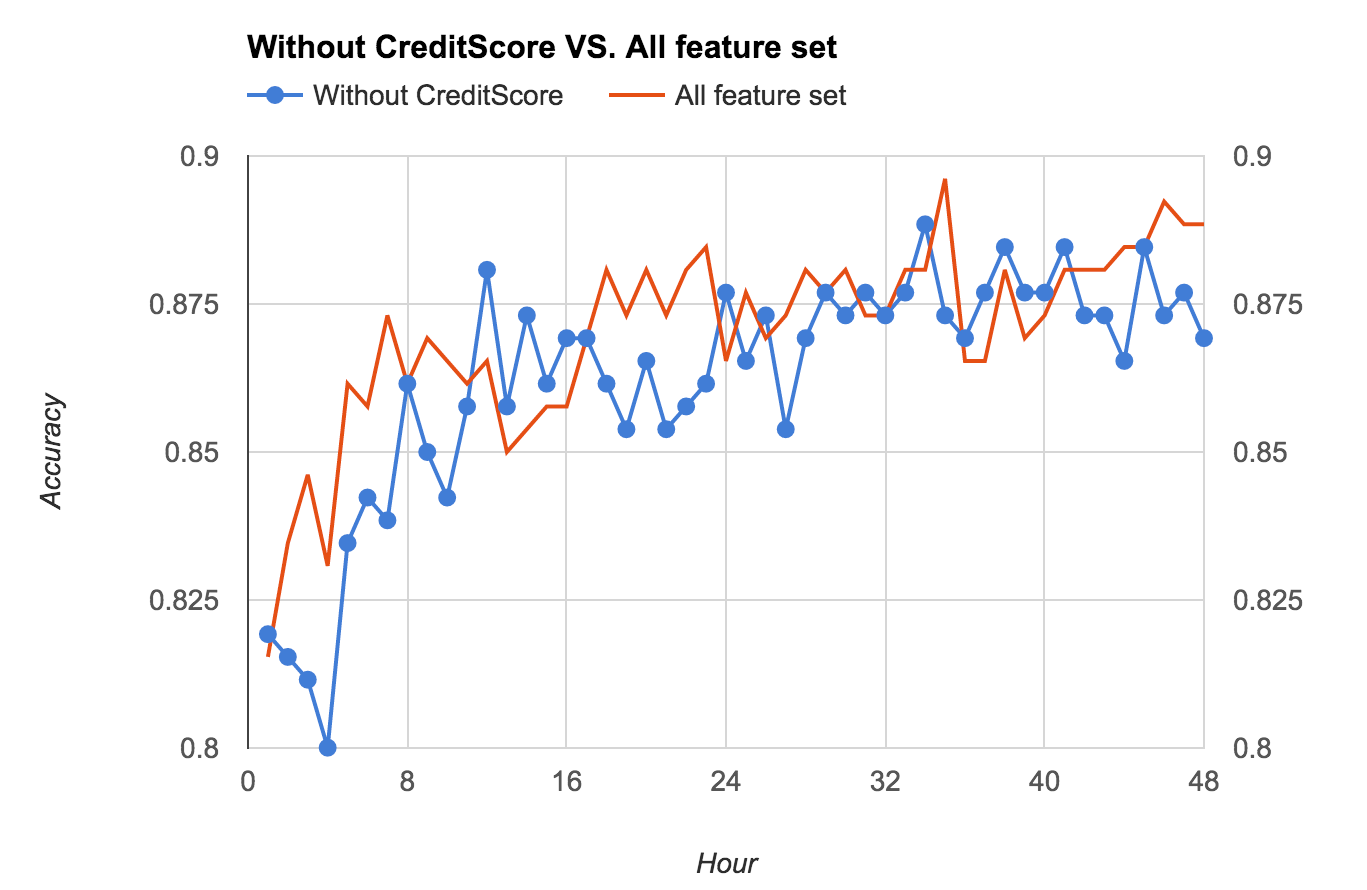
\includegraphics[width=\columnwidth]{images/WCVSAF.png}
\caption{Accuracy: Time series VS static Features}
\label{fig:WCVSAF}
\end{figure}

  \begin{table*}[!h]
 \centering
\scalebox{1}{
\begin{tabular}{@{\textbf{ }}cll@{}}
\toprule
\textbf{Hour} & \textbf{Rank} \\ \midrule
1 & 2\\
2			& 1\\
3			& 1\\
4			& 1\\
5			& 0\\ 
..  & 0\\ 
48 & 0\\ 
\bottomrule

\end{tabular}}
\caption{Ranks of CreditScore}
\label{tab:Rank_Credit}
\end{table*}
  
  
 \subsection{Crowd Wisdom} 
Crowd Wisdom is also a good feature which can get 75.8\% accuracy as a single feature. But its performance is very poor (less than 70\%) in the first 32 hours. The crowds need time to unify their views to the event after absorbing all kind of information. That is also one reason we need this automatic detecting system. 

 \subsection{Machine vs Human } 
 Our system is meaningless if the system detecting the rumors after the human recognize them. In this section we will compare our system with the human rumor debunking website snopes.com and urbanlegend.com. 
 
 Snopes.com has their own Twitter account \footnote{https://twitter.com/snopes}. They will post tweets via this account about rumors which they collected and verified. We consider the creation time of the first tweet which contains the keyword "snopes" OR "urbanlegend" in the tweets or URL of "snopes.com" is the time stamp of human confirming rumors. 


   But some of the rumors have a long duration, the website may report it several months ago or later the biggest burst peak. For example in figure \ref{fig:Multipike} it is a rumor about the rapper Tupac Shakur, who is thought to have been killed in 1996, is alive and comes out of hiding. This topic bursted in 2012, 2015 and 2016 several times and the tweet volume of 2012 is the highest so our $t_{max}$ is defined in 2012. But "snopes.com" reported this rumor in the september 2015\footnote{http://www.snopes.com/media/notnews/tupac.asp}. So we think that they don't refer to the same rumor affair.
  \begin{figure}[!h]
\centering
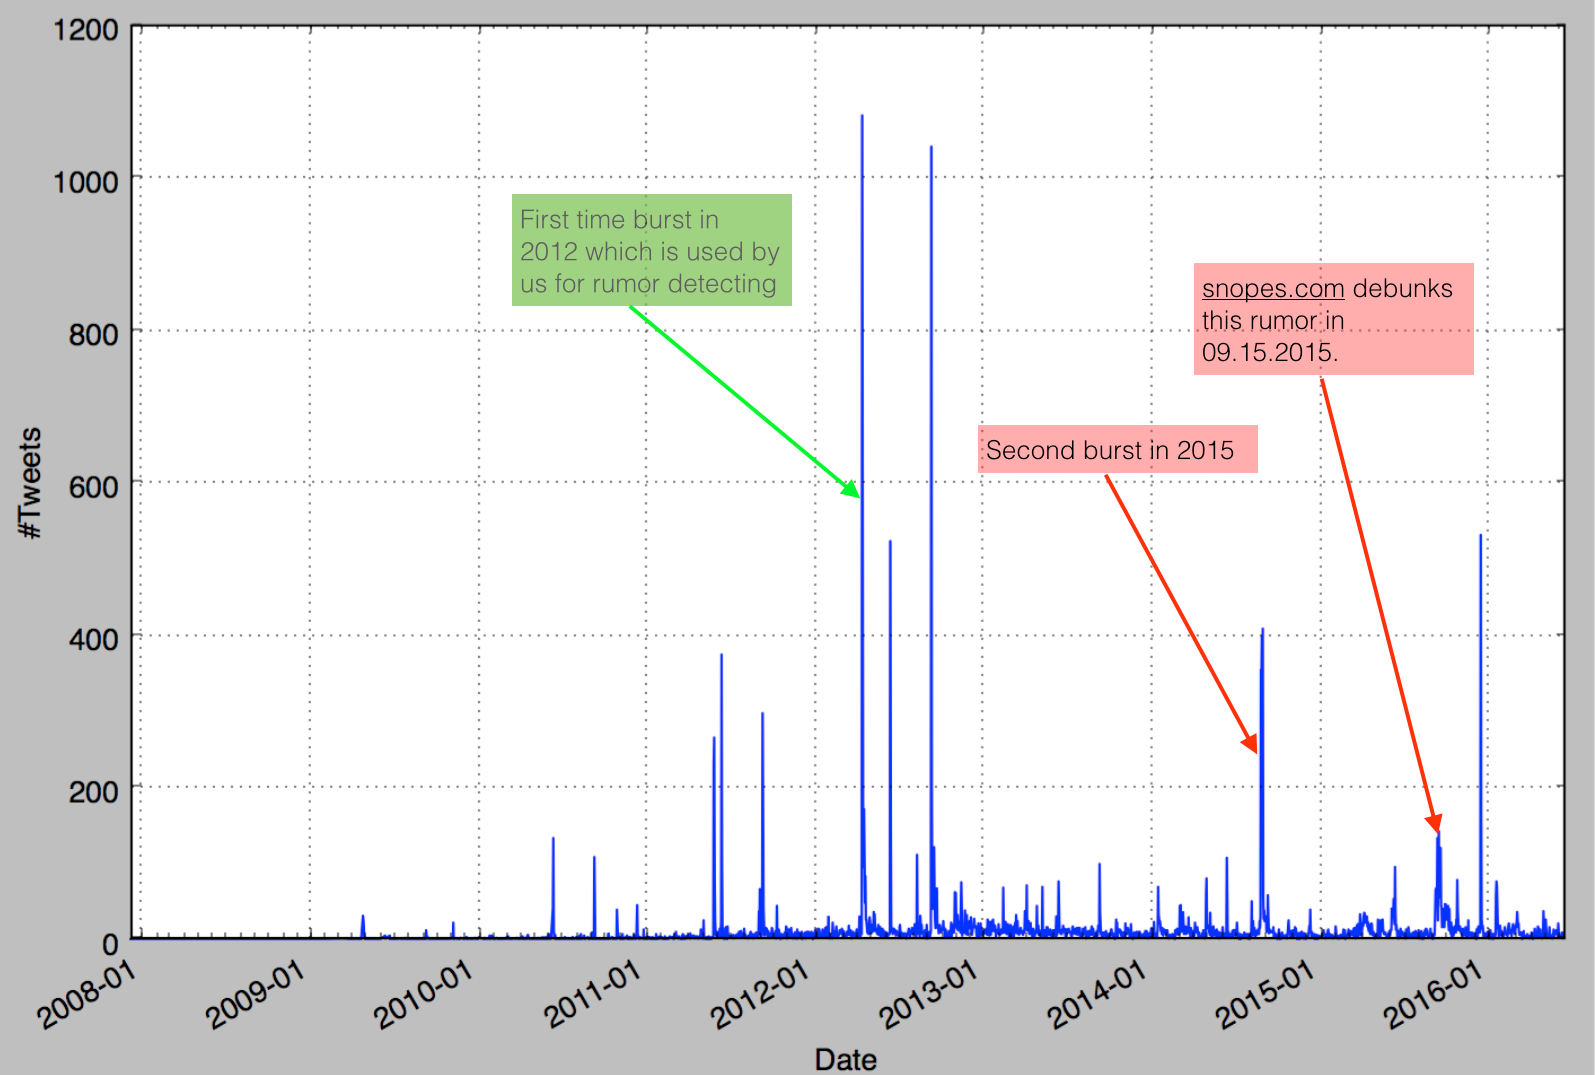
\includegraphics[width=\columnwidth]{images/mutipikehiding.png}
\caption{Tweet Volume Of Rumor about Tupac Shakur}
\label{fig:Multipike}
\end{figure}   
   
    So we set up a threshold 72 hours. We only consider the first tweet containing snopes keyword or snopes URL within 72 hours before or after the beginning time of the events which is defined in section \ref{sec:Time_Period_of_an_Event}. We show two examples here. First one in figure \ref{fig:ealiset_rumo} is a rumor about okra Curing diabetes\footnote{http://www.snopes.com/medical/homecure/okra.asp} which we detected the beginning time is 01.31.2014 04:00. So we scan the first tweet about snopes and we find it in 01.28.2014 21:00 which is 55 hours earlier than the beginning time. Snopes didn't explain their source of this rumor, maybe they detect the story not from Twitter. 
    Other example is in figure \ref{fig:lastest_rumo} is that  human detect rumor 71 hour after the event beginning.  
    The result is shown in table. On average the editors of "snopes.com" need 25.49 hours to verify the rumors and post it. Our system already achieves 87\% accuracy in 25 hours. 
     \begin{figure}[!h]
\centering
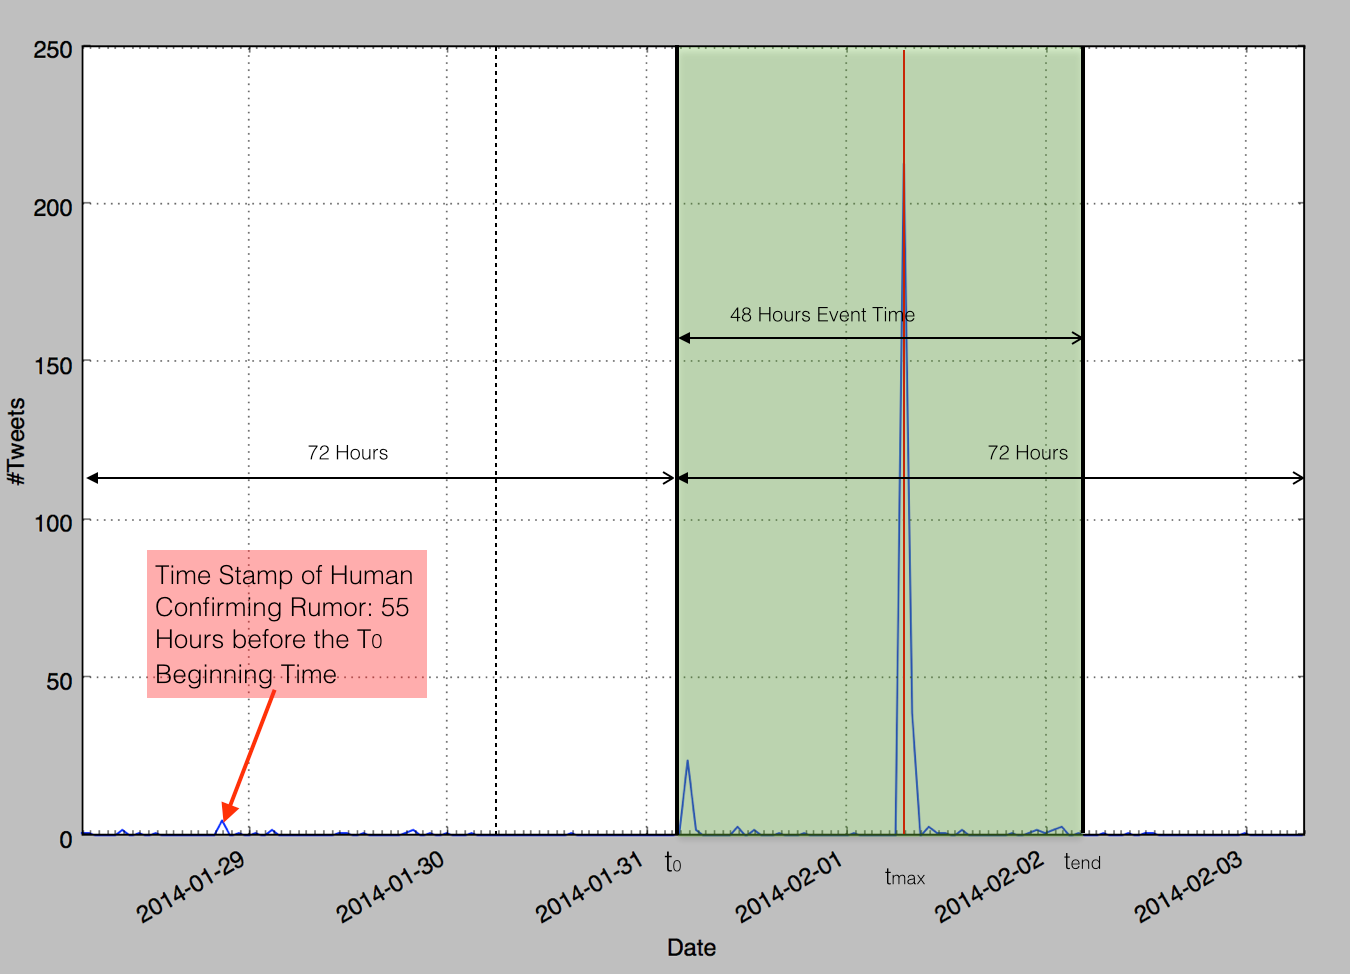
\includegraphics[width=\columnwidth]{images/Timestamphummanearlist.png}
\caption{The Earliest Time Stamp Of Human Confirming Rumor}
\label{fig:ealiset_rumo}
\end{figure} 
  \begin{figure}[!h]
\centering
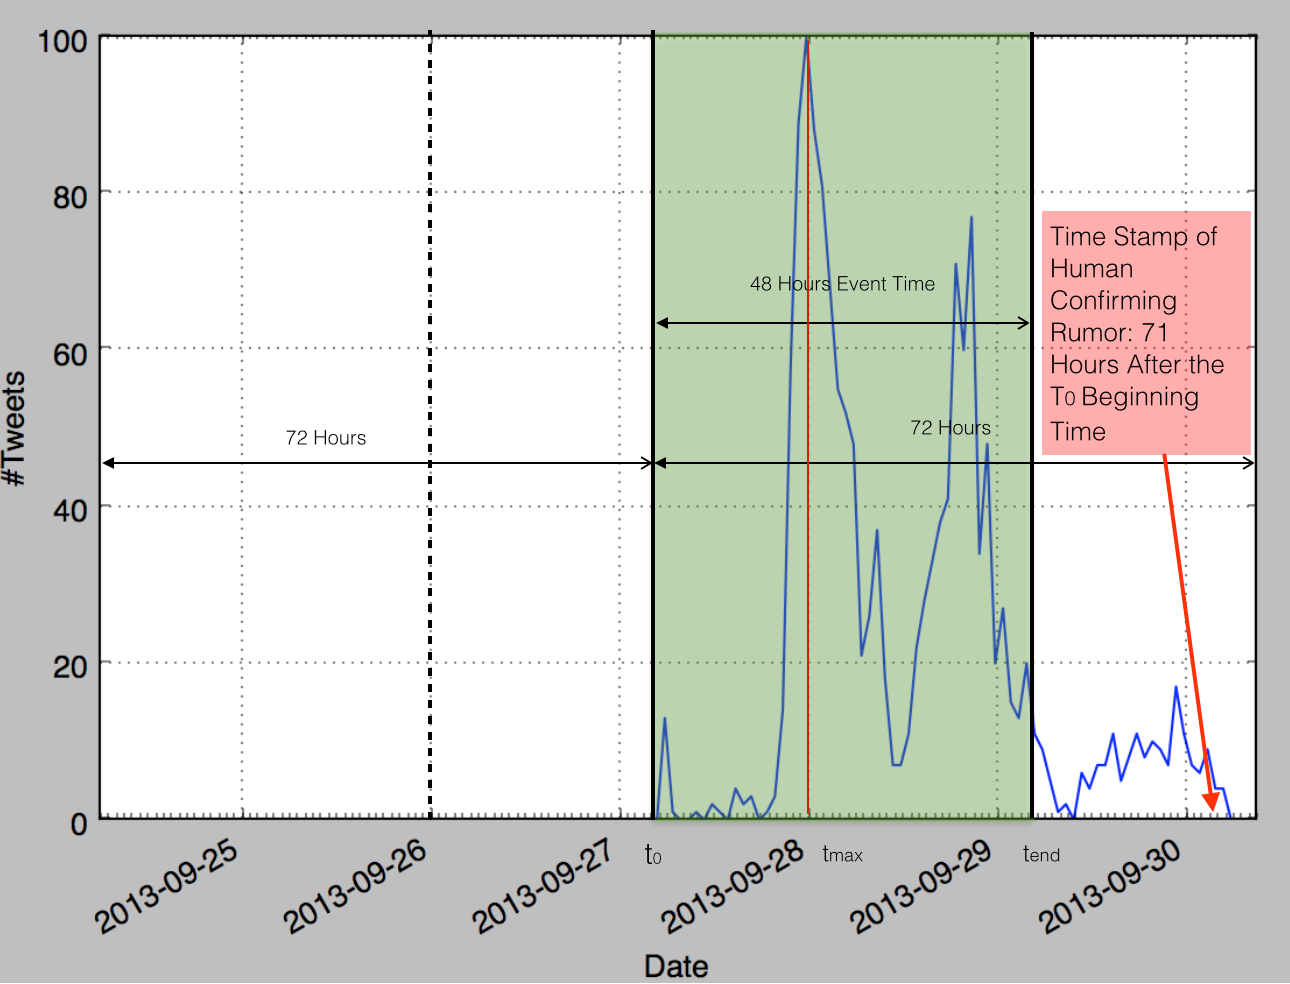
\includegraphics[width=\columnwidth]{images/Timestamphummanlatest.png}
\caption{The Lastest Time Stamp Of Human Confirming Rumor}
\label{fig:lastest_rumo}
\end{figure} 
  \begin{table*}[!h]
 \centering
\scalebox{1}{
\begin{tabular}{@{\textbf{ }}cll@{}}
\toprule
\textbf{} & \textbf{Hours} \\ \midrule
Latest Time of Human Detection & 71\\
Earliest Time of Human Detection			& -55\\
Average 		& 25.49\\
\bottomrule

\end{tabular}}
\caption{Time of Human Confirming Rumors }
\label{tab:Rank_Credit}
\end{table*}
 
 \clearpage
 \section{Discussion } 
 \subsection{Why sentiment doesn't work so well in time series model}
 \emph{PolarityScores} is the best feature of single tweet model. But it dose not work well in time series. Generally   the performance of \emph{PolarityScores} drops down over time. 
  In table \ref{Percentage-of-tweet-type} we reference the result from Thomas Heverin's work \cite{heverin2010microblogging}. He analyzed the tweets which responded to the 2009 Violent Crisis. The number of tweets containing original information and emotion are less and less over time. In the other hand more and more people start to share their different opinions even technology problems after 24 hours. That may make difference of sentiment features between rumors and news less and less in first 12 hours and after 24 hours it becomes useless. 
\begin{table}[!h]
\centering
\begin{tabular}{ccccccc}
\hline

\multicolumn{1}{|c|}{\small{Time Period}} & \multicolumn{1}{c|}{\small{Information}} & \multicolumn{1}{c|}{\small{Opinion}} & \multicolumn{1}{c|}{\small{Technology}} & \multicolumn{1}{c|}{\small{Emotion}} & \multicolumn{1}{c|}{\small{Action}} & \multicolumn{1}{c|}{\small{Other}} \\ \hline
\multicolumn{1}{|c|}{\small{0-12hours}}   & \multicolumn{1}{c|}{90.0\%}           & \multicolumn{1}{c|}{6.8\%}        & \multicolumn{1}{c|}{1.1\%}           & \multicolumn{1}{c|}{5.6\%}        & \multicolumn{1}{c|}{1.1\%}       & \multicolumn{1}{c|}{0.0\%}      \\ \hline
\multicolumn{1}{|c|}{\small{12-24 hours}} & \multicolumn{1}{c|}{86.6\%}           & \multicolumn{1}{c|}{13.0\%}       & \multicolumn{1}{c|}{3.1\%}           & \multicolumn{1}{c|}{4.5\%}        & \multicolumn{1}{c|}{1.3\%}       & \multicolumn{1}{c|}{0.7\%}      \\ \hline
\multicolumn{1}{|c|}{\small{24-36 hours}} & \multicolumn{1}{c|}{73.9\%}           & \multicolumn{1}{c|}{18.3\%}       & \multicolumn{1}{c|}{7.0\%}           & \multicolumn{1}{c|}{2.7\%}        & \multicolumn{1}{c|}{0.5\%}       & \multicolumn{1}{c|}{3.7\%}      \\ \hline
\multicolumn{1}{|c|}{\small{26-48 hours}} & \multicolumn{1}{c|}{74.6\%}           & \multicolumn{1}{c|}{21.3\%}       & \multicolumn{1}{c|}{1.0\%}           & \multicolumn{1}{c|}{3.8\%}        & \multicolumn{1}{c|}{0.5\%}       & \multicolumn{1}{c|}{2.8\%}      \\ \hline

\end{tabular}
   \caption{. Percentage of tweet type (non-exclusive) per 12 hour time period (source: \cite{heverin2010microblogging})}
\label{Percentage-of-tweet-type}

\end{table}


  \subsection{performance of external URLs features}
  In our experiment we have 3 features about the external URLs \emph{ContainNEWS}, \emph{UrlRankIn5000} and \emph{WotScore}. It is clear to see in table \ref{twitterfeaturerank} that after 24 hours the performances of these features are better than before 24 hours.    
  
  In Alexander's work \cite{mills2009web}, he also shows similar phenomenon that credibility of the information from twitter is higher than external website in the first 24 hours \ref{fig:informationqulitat}. 
  \begin{figure}[!h]
\centering
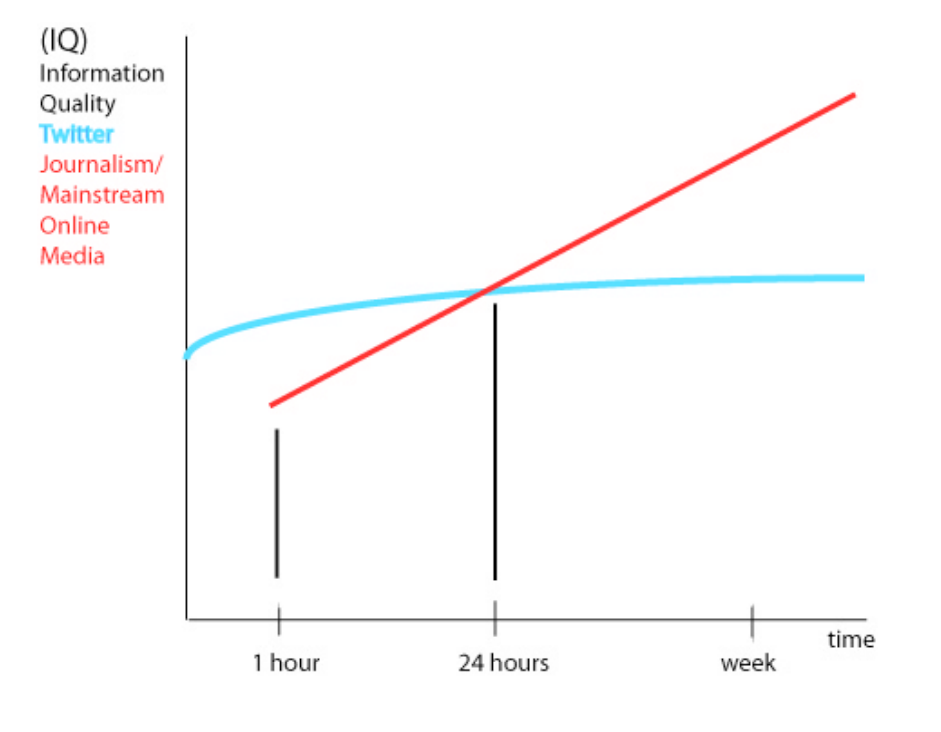
\includegraphics[width=0.7\columnwidth]{images/Informationqulitat.png}
\caption{Information Quality over time (source: \cite{mills2009web})}
\label{fig:informationqulitat}
\end{figure}
\newpage
That may be the reason why the features of external links need 24 hours to performance better.
 \section{Case Study: Munich Shooting } 
At 17:52 CEST a shooter opened fire in the vicinity of the Olympia shopping mall in Munich. 10 people, including the shooter, were killed and 36 others were injured\footnote{https://en.wikipedia.org/wiki/2016\_Munich\_shooting}. 

At 18:22 first tweet was posted. It might contain some delay here, because our query is constructed in English and maybe the very first tweets are in german language. The tweet is "Sadly, i think there's something terrible happening in \#Munich \#Munchen .  Another Active Shooter in a mall. \#SMH". 3 minutes later at 18:25 the second tweet was posted: "Terrorist attack in Munich????". Both of them are labeled by the single credit model as news related.  

At 18:27 the traditional media (BBC) posted their first tweet. "'Shots fired' in Munich shopping centre - http://www.bbc.co.uk/news/world-europe-36870800a02026 @TraceyRemix gun crime in Germany just doubled".

The first misclassification tweet is at 18:31. It was a tweet with shock sentiment and swear words. "there's now a shooter in a Munich shopping centre.. What the fuck is going on in the world. Gone mad"

We show the credit score of Munich attack event in figure \ref{fig:munichattackCS}. It is clear to see that the credit score of Munich Shooting is below the average of news.  
  \begin{figure}[!h]
\centering
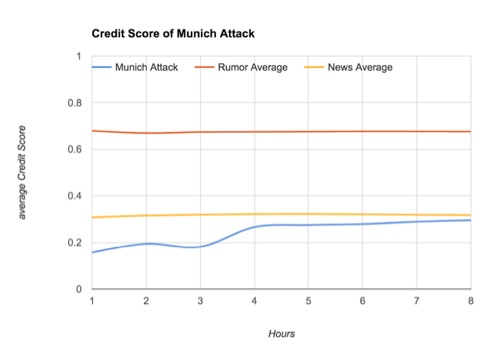
\includegraphics[width=0.7\columnwidth]{images/munichCD.png}
\caption{Credit Score of Munich Shooting}
\label{fig:munichattackCS}
\end{figure}

And there are several kinds of misclassification in table 
\ref{tab:Munshot}: 
unrelated to the events, strong emotional and rumor related.
We searched the tweet in English, so most of user are in America not in Germany which can talk about some extend topic like gun law. These comments are labeled as rumors by our system. And some tweets contain strong personal emotion even swear words. These tweets have higher probability being labeled as rumor. The third type is rumor. Some rumors were spreading with the news events. For example some tweets claimed Sam Hyde was the shooter and posted a photo in which there is a man with gun. Or some claimed the shooter was member of ISIS. They are also detected by our system. But generally the average credit score is more like a news event.  
\begin{table*}[!h]
 \centering
\scalebox{1}{
\begin{tabular}{@{\textbf{ }}cp{350pt}@{}}
\toprule
\textbf{Catalogue} & \textbf{Examples of Tweets} \\ \midrule
\multirow{2}{*}{Event Unreleted} & Looks like the EU's gun ban has continued to do its job. What a success. \#Munich https://twitter.com/RT\_com/status/756525863093538817\\\cline{2-2} 
 			& The strict gun laws in Munich kept guns out of innocent hands, didn't stop the terrorists, in fact made their job easier. @realDonaldTrump\\\cline{2-2}
 	&	@KummersTim @ShepNewsTeam Shep Smith is colluding with Hillary's camp also what he tried during Munich attack was disgusting \#TrumpPence16	\\
 			\midrule
\multirow{2}{*}{Strong Emotional}  & Munich Another day another attack. when is this shit gonna end. It is becoming the norm now. Saddening .\\ \cline{2-2} 
 			& there's now a shooter in a Munich shopping centre.. What the fuck is going on in the world. Gone mad\\\midrule
Rumors			& ISIS On Munich Terror Attack: Everything Hurting Infidels Makes Us Happy http://www.weaselzippers.us/285113-isis-on-munich-terror-attack-everything-hurting-infidels-makes-us-happy/ via @WeaselZippers\\ \cline{2-2}
			& Obama released photo of shooter \#Munich pic.twitter.com/GzJkyNpYDP\\\cline{2-2}
			& Nice attack 7 days ago, Wurzburg axe attack Monday, Alps knife attack on Wednesday \& Munich shootings ongoing. All are Jihad, get used to it\\\cline{2-2}
			& New info: Munich shooter has been consuming high amounts of a chemical substance called \"H2O\"! \#banH2O \#banChemistry \\\cline{2-2}
			& @M7madSmiry @TheBpDShow hearing reports that the shooter is a white supremacist... Has that been confirmed? \#Munich\\\cline{2-2}
			& Witness In Munich Shooting Says: The Shooter Cried Out Allahu Akbar As He Slaughtered Children http://shoebat.com/2016/07/22/witness-in-munich-shooting-says-the-shooter-cried-out-allahu-akbar-as-he-slaughtered-children/  via @walidshoebat\\\midrule
others &	@ThatTimWalker seems you were wrong re the Munich attack.\\
		
 			\bottomrule

\end{tabular}}
\caption{Example of Misclassification by Single Tweet Model on Munich Shotting}
\label{tab:Munshot}
\end{table*}
  \begin{figure}[!h]
\centering
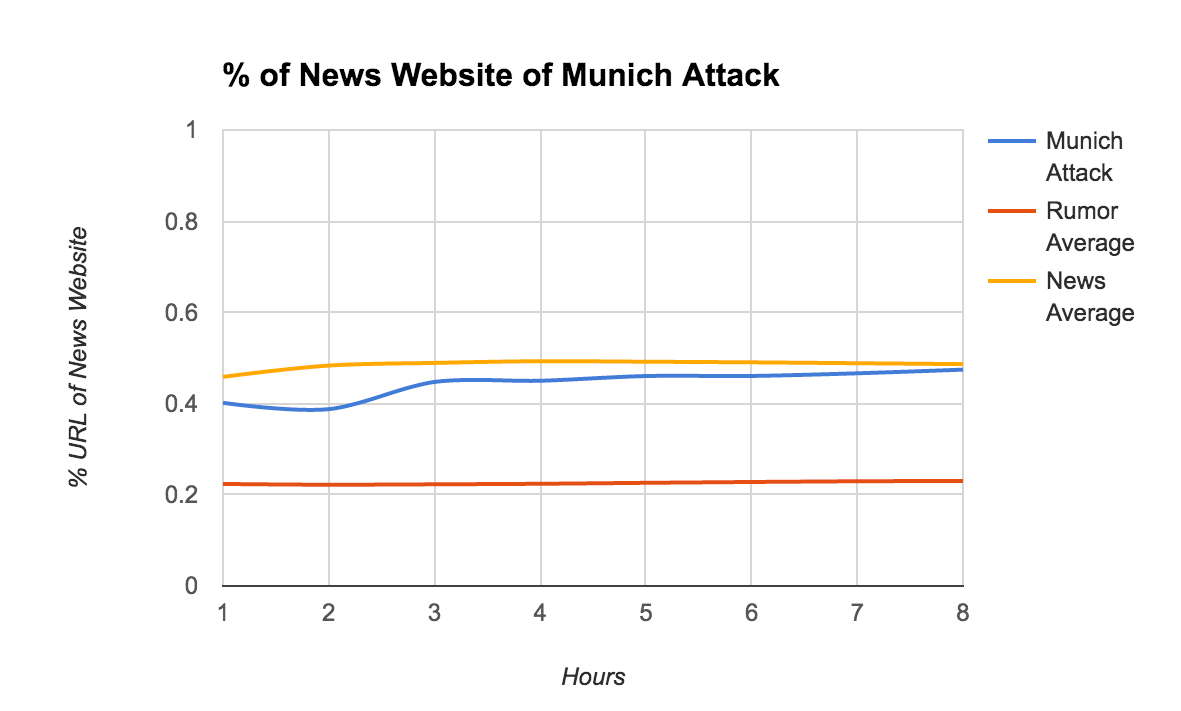
\includegraphics[width=0.8\columnwidth]{images/munichNews.png}
\caption{\% of Tweet Containing News Websites of Munich Shooting}
\label{fig:munichattackNews}
\end{figure}

The second best feature is ContainNews which is the percent of the URLs of tweet containing News Website domain. We are showing the ContainNews of Munich attack in figure \ref{fig:munichattackNews}. 
 We can see the curve of ContainNews of Munich shooting event is close to the curse of ContainNews average News events. 
 
 Our 
